\documentclass[arial,11pt]{article}
%\documentclass[11pt]{nih}
\usepackage[dvips]{graphicx}
\usepackage[colorlinks=true,linkcolor=black]{hyperref}
\usepackage{amsmath}
\usepackage{amssymb}
\usepackage{graphicx}
%\usepackage{longtable}
\usepackage{epsfig}
%\usepackage{overcite}
%\usepackage{lscape}
\usepackage{rotating}

\renewcommand{\rmdefault}{phv} % Arial
\renewcommand{\sfdefault}{phv} % Arial
\renewcommand{\thesection}{\Alph{section}}
\pagestyle{empty}

%\usepackage{times}
\usepackage{geometry}
%\geometry{tmargin=1in,bmargin=1.0in,lmargin=1in,rmargin=1in}
\geometry{tmargin=0.95in,bmargin=0.95in,lmargin=0.95in,rmargin=0.95in}
%\linespread{0.95} \interfootnotelinepenalty=10000

%%%%% editing helpers
\newcommand{\NeedRevision}[1]{\textcolor{red}{#1}}
\newcommand{\speclib}{\ensuremath{\mathcal{L}}}
\newcommand{\ndp}{\ensuremath{ndp}}

\begin{document}

\begin{center}
{\Large {\bf Technology and Research Development Project 7: \\
Identification of multiplexed spectra}}
\end{center}

\section{Specific aims}
The complexity and dynamic range of compounds in proteomics samples is very large and continues to pose significant challenges for traditional data dependent acquisition (DDA) workflows, requiring long run times, replicate runs and very high speed MS/MS acquisition to deeply interrogate the samples. Data independent acquisition (DIA) strategies have been used to increase the reproducibility and comprehensiveness of data collection but mass spectrometry (MS) instruments have been limited in the speed and quality of the data they acquire. However, recent developments  have now made it possible to perform DIA with high speed and high resolution in  both MS and MS/MS modes~\cite{chakraborty2007uim,Gillet12targeted}. With sensitivity and dynamic range comparable to Selected Reaction Monitoring assays~\cite{Gillet12targeted}, these developments have the potential to unify quantification and identification while dramatically expanding the sensitivity and reproducibility of proteomics experiments in the detection of splice variants, low abundance proteins and post-translational modifications (PTMs). But despite the enormous potential of DIA approaches, almost all MS algorithms make the assumption that each spectrum is generated from only one analyte and thus cannot identify DIA multiplexed spectra - limitations that will require rethinking current algorithms and the development of new algorithmic ideas specifically for multiplexed spectra. We aim to develop tools that can identify multiple peptides from the same multiplexed spectrum.

\begin{itemize}
    \item {\bf Aim 1: Spectral library search of multiplexed spectra.} Spectral library search has been recognized as a more sensitive method (as compared to database search methods) for peptide identification from MS/MS spectra due to the fact that spectral libraries have more information about the actual fragmentation pattern of a particular peptide~\cite{zhangunderstanding}.  Given the inherent difficulties in identifying peptides from multiplexed spectra, it is expected that extending spectral library search to multiplexed spectra will significantly improve peptide identification rates.
        %Recently there are also growing availability of libraries of single-peptide spectra in public repositories. Thus
        We aim to develop a spectral library search method for peptide identification by modeling each multiplexed spectrum as a combination of spectra in the library.

    \item {\bf Aim 2: Database search of multiplexed spectra.} While there is a growing availability of peptide spectral libraries in the public domain, library search methods still suffer from the limitation that if a peptide has not been identified before, it cannot be identified using current library search approaches. While we expect that spectral library search tools will be more sensitive for identification of multiplexed spectra when the peptides are present in the library, we also aim to develop a database search method for identification of multiplexed spectra. %to address cases when the peptides in the multiplexed spectra are not represented in the spectral library.

     \item {\bf Aim 3: Computing statistical significance of multiPeptide-Spectrum Matches (mPSMs).} Calculation of false discovery rates (FDR) for multiplexed spectra containing different numbers of peptides of varying length remains an open problem.  In addition, it is important to be able to estimate the statistical significance of individual mPSMs, regardless of the number of other mPSMs also identified in a given dataset (as estimated by FDR). We propose to address these challenges by extending the generating function approach~\cite{kim2008spectral} developed at CCMS from single-peptide spectra to multiplexed spectra.

\end{itemize}

%*******************************************
\section{Significance}
%*******************************************

Over the past several years there have been substantial advances in the sensitivity of protein identification thanks to technological developments in chromatography and tandem MS.  In shotgun proteomics, researchers can routinely identify thousands of proteins from complex biological samples in a single experiment \cite{washburn2001,brunner2007high,aebersold2003mass}. But, despite this rapid progress, there are still challenging issues that remain unresolved \cite{chalkley05comprehensive,wenner2004factors}.  One such challenge is that in any high throughput MS/MS experiment only a fraction of MS/MS spectra can be identified by current computational methods.  While there are many factors contributing to this low spectrum identification rate, recent studies suggest that one reason is the occurrence of co-eluting peptides.  As instruments with high mass accuracy enable us to better distinguish peptides with close precursor masses, it was recently shown that as many as 50\% of the MS/MS spectra collected in typical proteomics experiments come from more than one peptide precursor~\cite{gelio2008detection,pr101060v,pr800307m,houel2010quantifying}, giving rise to \emph{multiplexed} spectra.  These spectra can confuse current computational methods because most  mainstream approaches make the assumption that each spectrum comes from a single peptide. Houel et. al., 2010~\cite{houel2010quantifying} demonstrated that the identification rates for multiplexed spectra are significantly reduced as compared to  spectra from single peptides~\cite{houel2010quantifying}.  Thus, computational methods that can handle multiplexed spectra can readily improve our ability to analyze spectral data in traditional experimental workflows.

More importantly, in recent years there have been numerous developments in DIA technologies where multiple peptide precursors are intentionally selected for co-fragmentation in each MS/MS spectrum~\cite{venable2004aaq, masselon2003itp, chakraborty2007uim, michalski2011mass,Gillet12targeted}.  Recent improvements in instrumentation have made it possible to perform DIA with high speed and high resolution in both MS and MS/MS modes. With continuing improvements in sensitivity and dynamic range, these emerging technologies can address some of the major disadvantages of traditional DDA methods (such as data reproducibility) and can potentially increase the throughput of peptide identification by 10--20-fold \cite{michalski2011mass,blackburn2010}.

However, despite the growing importance and the enormous potential of multiplexed spectra, there is still a shortage of computational methods to analyze them. In pioneering work, Zhang et al., 2005~\cite{zhang2005tree} described the first database search method for multiplexed spectra
%, ProbIDtree,
and showed that it is possible to identify co-eluting peptides from single MS/MS spectra.
However, their method typically
% in that study not all peptides could be confidently
identifies
%and in most cases ProbIDtree only identified
only the most prominent peptide in each multiplexed spectrum and
%. In addition, ProbIDtree's
its accuracy in identifying multiplexed spectra is relatively low
as compared to the accuracy of standard MS/MS database search tools in  identifying single-peptide spectra~\cite{wang2011peptide}.  Other methods approach the multiplexed spectra identification problem by reporting spectra with more than one significant single-peptide match and do not explicitly attempt to model the occurrence of fragment ions from more than one peptide in the same spectrum.  False Discovery Rates (FDR) are also left unadjusted~\cite{zhang2005tree,kall2007semi,bern2007lookup} and may result in inflated FDR for multiplexed spectra (e.g., when co-eluting peptides share a substantial number of fragment masses).  Finally while much attention has been dedicated to computing the statistical significance of a PSMs for single-peptide spectra~\cite{nesvizhskii2010,gupta11}, this fundamental question still remains  unanswered for multiplexed spectra. This TRD will address these challenges in identifying multiplexed spectra.
%By focusing on the special case of multiplexed spectra that comes from two peptides, recently we proposed a spectral-library search method, M-SPLIT~\cite{wang2010msplit} and a new database search method, MixDB~\cite{wang2011peptide}, and show that mmultiplexed spectra can be identified efficiently with comparable accuracy to that of single-peptide spectra.


%*******************************************
\section{Innovation}
%*******************************************
One of the main challenges in identifying multiplexed spectra is the combinatorial explosion of the search space of candidate peptides that can be matched to a multiplexed spectrum. We address this challenge by first using filtration techniques based on the concept of {\em projected spectrum}, which can reduce the search space of candidate peptides by several orders of magnitude.  Using efficient search methods such as branch-and-bound techniques, greedy search algorithms and Linear Programming (LP),  we show that it is possible to identify multiplexed spectra by only considering a small fraction of the total search space.

Our approaches also introduce new probabilistic scoring models for matching multiple peptides against a multiplexed  spectrum.  While many approaches have been explored for designing scoring functions for PSMs, very few methods can handle the case of more than one peptide per spectrum. Even in search tools that can handle multiple peptide matches per spectrum, they often borrow the same scoring models from single-peptide spectrum. However, we observe that peptides with different relative abundances (at the time of MS/MS co-acquisition) have quite distinct MS/MS peptide fragmentation characteristics and thus scoring models trained from single-peptide spectra become inadequate  for multiplexed spectra. We propose a scoring function to take this into account by $i)$ having different fragmentation models for different relative peptide abundances and $ii)$ modeling the dependencies among different peptide candidates in each multiplexed spectrum.  The latter is important because otherwise peptide candidates that share a large fraction of theoretical fragment ions will most likely be scored with an artificially high score.

Peptide identification tools need to be accompanied by methods for the accurate calculation of the statistical significance of a PSM.  This is especially crucial for multiplexed spectra because of the  vast space of possible candidate peptide mixtures, which dramatically increases the chances of randomly obtaining high-scoring false positive matches.  We propose to extend the MS-GF~\cite{kim2008spectral} algorithm and rigorously compute the statistical significance for multiPeptide-Spectrum-Matches (mPSMs).  While preliminary results indicate that this approach improves sensitivity in identification of multiplexed spectra, it is also computationally expensive. We will address this shortcoming by proposing an alternative approximation approach that efficiently computes the statistical significance of mPSMs.
%Finally, we will also extend the traditional target-decoy-approach (TDA) to calculate the false discovery rate (FDR) for multiplexed spectra.

%--Model of multiplexed spectra in term of single-peptide spectra\\
%--Filtration strategy: concept of projected spectrum\\
%		--Relative quantification of peptide abundance in multiplexed spectra\\
%--Scoring models for co-fragmentation of multiple peptides in multiplexed spectra\\
%--Computing statistical significance of peptide-spectrum-match in multiplexed spectra \\
%--FDR estimation of multiplexed spectra \\
%--

%*******************************************
\section{Approach}
%*******************************************

% Published results and updates

\subsection{Aim 1: Spectral library search of multiplexed spectra}

\subsubsection{\bf Identification of multiplexed spectra from two peptides.}

To introduce the proposed approach for multiplexed spectra, we first explain the logic of our M-SPLIT  algorithm~\cite{wang2010msplit}. While  M-SPLIT considers only the special case where the multiplexed MS/MS spectrum comes from only two peptides, the computational ideas behind M-SPLIT are important for this TRD.
Moreover, this simple case accounts for a large fraction of multiplexed spectra present in traditional DDA workflows~\cite{pr800307m} and thus allows us to develop algorithmic concepts using DDA (since data from DIA workflows is still not widely available). After introducing M-SPLIT, we will describe how to extend this approach to the multiplexed spectra from more than 2 peptides.
%In brief, a multiplexed spectrum is modeled as linear combination of two single-peptide spectra and peptide identification is done by searching against a spectral library to find the best matching pair. We show that efficient filtration and accurate branch-and-bound strategies can be used to avoid the huge computational cost of searching all possible pairs. Thus equipped, our approach is able to identify the correct matches by considering only a minuscule fraction of all possible matches.

%A multiplexed spectrum is defined as a spectrum from two different peptides.
% and a spectral library is a collection of identified MS/MS spectra.
%Analogous to the identification of MS/MS spectra by comparison against a database of known protein sequences, our %goal is %to
M-SPLIT identifies multiplexed spectra by comparison against a spectral library.
Similarly to other CCMS tools (see TRD4 and TRD5), a  spectrum is represented as a vector of $n$ bins, each representing a mass interval of width $\delta$ (where $\delta$ depends on instrument resolution).  A bin has value zero if there are no peaks in the corresponding $\delta$-Dalton interval, otherwise it is the summed intensity of all peaks whose masses fall in that bin.  We model a multiplexed spectrum $M$ as $M \approx  A+\alpha B$, where $A$ and $B$ are single-peptide MS/MS spectra from two different peptides and $\alpha$, the mixture coefficient, indicates their relative abundance in $M$. Without loss of generality, we assume that $A$ and $B$ are scaled to Euclidean norm 1 and that $0\leq\alpha\leq 1$ (i.e., $A$ corresponds to the higher abundance peptide).  To measure how well $A+\alpha B$ approximates $M$, we need to  define {\em similarity} between two peptide spectra~\cite{atwater1985,craig06,lam2007}. Below we  use the widely accepted {\em normalized dot product} (cosine) measure of spectral similarity.
We now formulate the following  problem:\\

\begin{tabular}{ll}
\multicolumn{2}{l}{\textbf{Multiplexed Spectrum Identification Problem (MSIP)}}\\
\textbf{Input}  & A mixture spectrum $M$ and a spectral library \speclib.\\
\textbf{Output} & A constant $0\leq\alpha\leq 1$ and a pair of spectra ${A,B}\in\speclib$ maximizing $similarity(M,A+\alpha B)$\\
\end{tabular}\ \\

%While there are several ways to define similarity between two peptide spectra~\cite{atwater1985,craig06,lam2007}, %we chose to use the normalized dot product or cosine measure of spectral similarity is widely accepted to be a robust %measure.

%{\bf Simulation of Multiplexed Spectra.} Since there is currently no publicly available data with validated identifications of mixture MS/MS spectra, we constructed a dataset of simulated mixture spectra to benchmark our approach.
%% we used the MS/MS spectral library from the National Institute of Standards and Technology (NIST). %All spectra in %the library are first scaled to Euclidean norm 1. Since in a multiplexed spectrum the two peptides will most likely be %present at different abundances,%
%Multiplexed spectra were simulated by randomly selecting two spectra from the NIST spectral library and linearly combining them using a predefined mixture coefficient
%%$\alpha$.  Below we benchmark our approach for
%$\alpha\in\{0.1-1.0\}$ (see ~\cite{wang2010msplit} for details).
%%To simulate signal suppression, the final simulated multiplexed spectrum was filtered by retaining only the 10 most %intense peaks in a window of 50~Da.

{\bf Projected spectra.} While the MSIP formulation is simple, the rapidly growing size of spectral libraries (already on the order of $10^6$ spectra~\cite{NIST}) makes searching all possible {\em pairs} of spectra prohibitively time-consuming. M-SPLIT  avoids this quadratic search time by (i) using a {\em projected-cosine} filter to eliminate a large fraction of spectra in the library, and (ii) using a {\em branch-and-bound strategy} to limit the search for the best-matching pairs to only a subset of all possible pairs.
%The full algorithm is described in reference~\cite{wang2010msplit}, we will outline the core concepts below.

While cosine is generally a good measure of spectrum similarity, a multiplexed spectrum ${M}$ derived from peptides $A$ and $B$ may have limited similarity to the corresponding single-peptide spectra - e.g, the presence of ${B}$ in the mixture may result in many unmatched peaks between ${M}$ and ${A}$.  We address this issue with the concept of {\em projected-spectrum} \cite{wang2010msplit}. For two vectors $A$ and $M$, the projection $M_{A}$ of $M$ on $A$ is defined as:
\begin{eqnarray*}
	M_{A}[i] = \left\{ \begin{array}{ll}
                     M[i] & \mbox{if\ } A[i] > 0\\
                     0    & \mbox{otherwise}\\
                     \end{array}
                  \right.
\end{eqnarray*}
The projected cosine between $M$ and $A$ is then simply the cosine between	$M_{A}$ and $A$:
\begin{eqnarray*}
	\cos_{p}(M, A) = \frac{{	M_{A}}\cdot{A}}{\left\|{	 M_{A}}\right\|\left\|{A}\right\|}
\end{eqnarray*}

The intuition behind this operation is that since spectrum  $A$ contains all observed fragment ions from peptide A, the projection essentially separates the peaks that are possibly generated from peptide A from those that are noise or generated from peptide B in the multiplexed spectrum.
Given a spectrum $M$, the filtering step consists of computing the projected-cosine similarity between $M$ and all spectra in \speclib\ and retaining the top K most similar matches.  The filtering efficiency can be determined by how large K need to be.
% and as shown in Figure~\ref{Psimranks}a,
As shown in \cite{wang2010msplit}, in more than $95\%$ of cases we only need to consider the top $500$ candidates in a library, even though for cases with high $\alpha$ only $\leq 100$ candidates are typically required.
% with 27,966 candidates.

%The branch-and-bound strategy involves deriving a $UpperBound(M,A)$, that determine the maximum cosine similarity that any pair of spectra that contains $A$ can achieve when matched to $M$.  Thus, during certain stage of the search, any spectra with $Upperbound$ less than the current best cosine similarity will not be considered.
%%The search efficiency of the branch-and-bound and the overall M-SPLIT algorithm is shown in %Figure~\ref{Psimranks}b and c.\\
%During the search, we need to quickly compute the mixture coefficient $\alpha$. As shown in  \cite{wang2010msplit} the following estimate of the mixture coefficient works well:
%
%\begin{eqnarray*}
%	%\hat{\alpha} = \frac{AE-CD}{BC-DE}
%	\hat{\alpha} = \frac{M\cdot B - (M \cdot A)(A \cdot B)}
%	{M\cdot A - (A\cdot B)(M\cdot B)}
%\end{eqnarray*}

%\begin{figure}[htpd!]
%	\centering
%		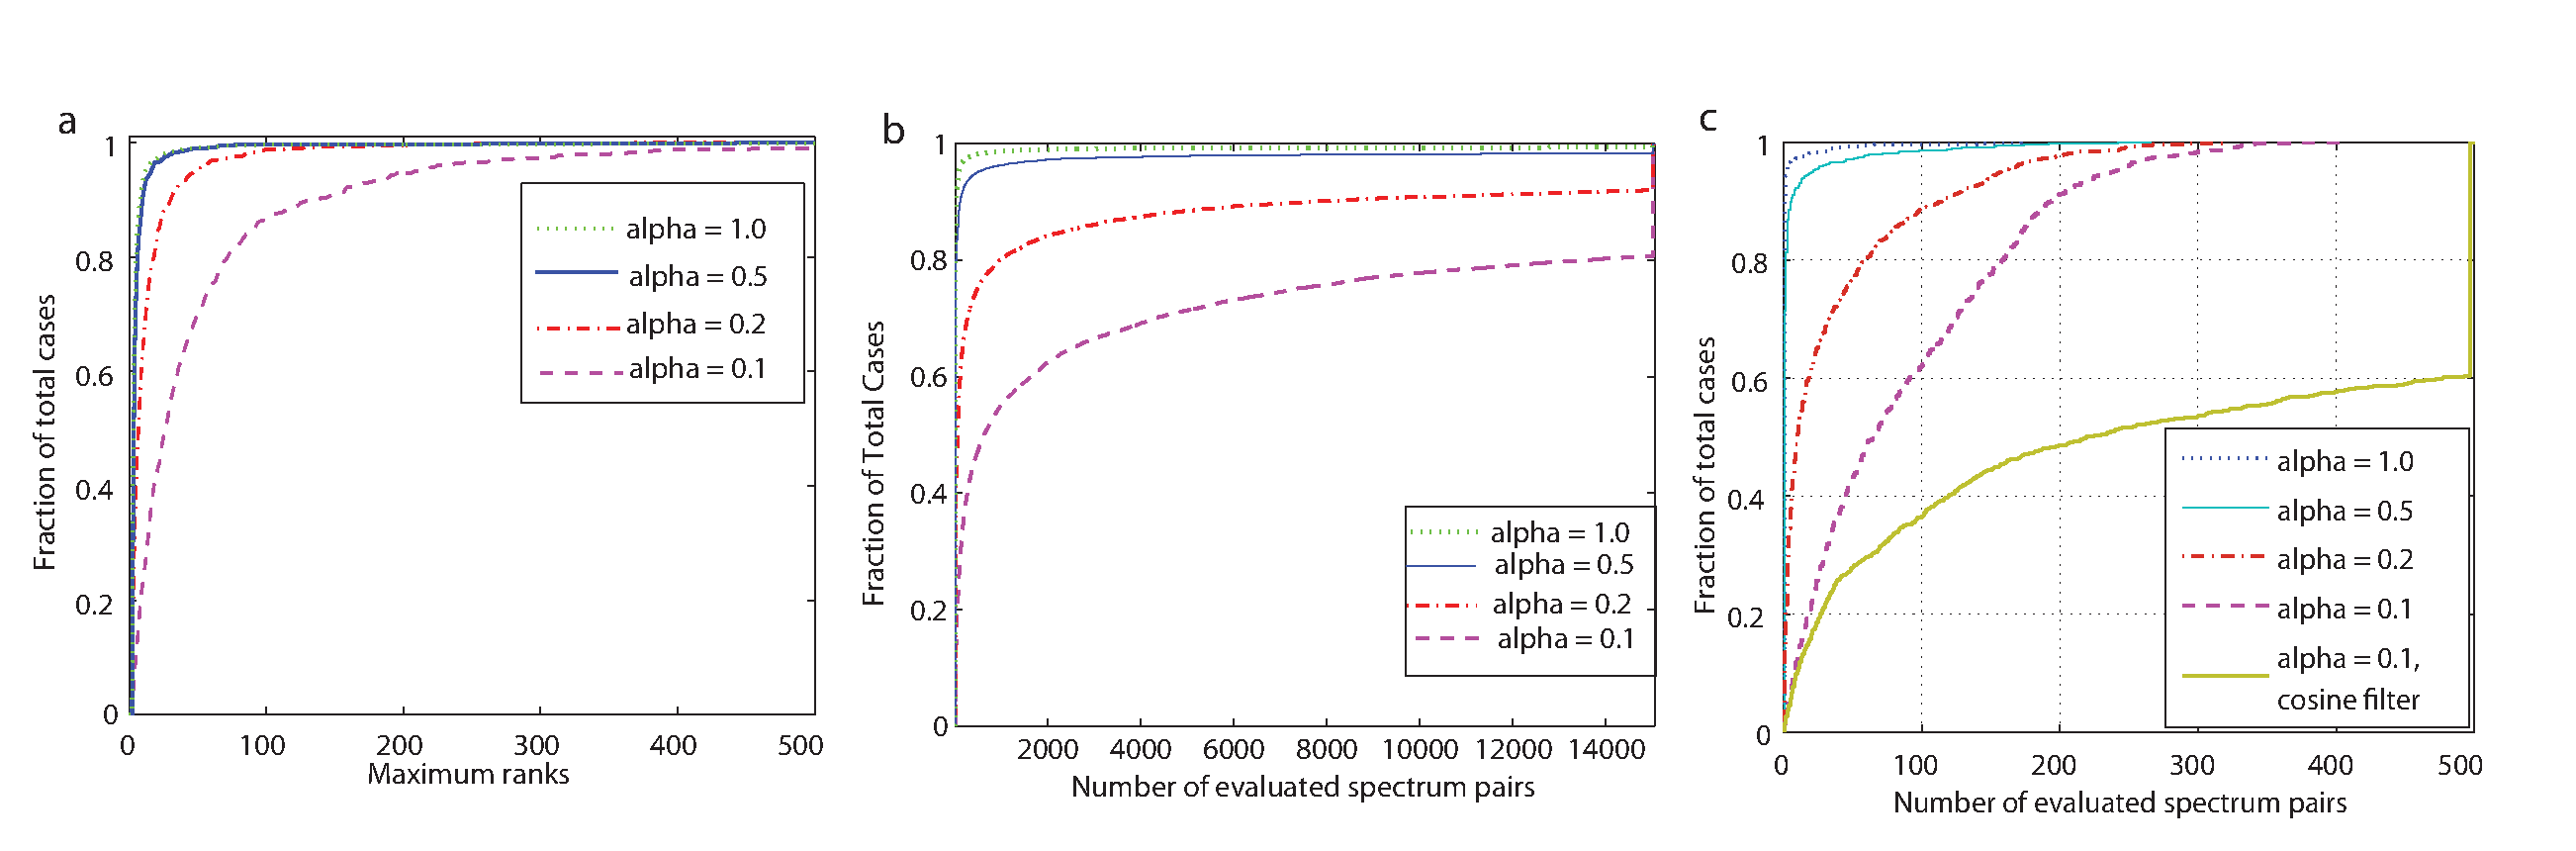
\includegraphics[height=60mm, width=170mm]{Figures/MSPLIT_efficiency_reformat}
%		\caption{M-SPLIT search efficiency: {\footnotesize \textbf{a)} Cumulative distributions of maximum rank for correct matches to the spectral library. Spectra in the library are first sorted according to decreasing projected-cosine similarity to the multiplexed spectrum (library containing 27,966 spectra). The rank of correct matches are then determined. Correct matches are spectra identified as one of the peptides in the multiplexed spectrum. Since each multiplexed spectrum has two correct matches (it is generated from two peptides) we take the maximum (i.e., worst) rank of the two matches.
%\textbf{b)} To avoid considering all {\em pairs} of spectra in the library, we derive a branch-and-bound search strategy to eliminate a large fraction of all possible pairs. The number of evaluated pairs of spectra is shown. Since the total number of possible pairs is $3.9 \times 10^{8}$ and our approach never evaluates more than 15,000 pairs, this self-adjusting strategy achieves speedups of at least $2 \times 10^{4}$. \textbf{c)} Combining the projected-cosine filter (part a) with branch-and-bound search (part b): we first filter the spectral library with projected-cosine and retain only the top 500 candidates; the branch-and-bound search strategy is then applied to further reduce number of pairs of spectra that needed to be evaluated.  The combined filters typically achieve speedups of approximately six orders of magnitude ($\approx\frac{3.9 \times 10^{8}}{500} = 7.8 \times 10^{5}$ speedups).}}
%	\label{Psimranks}
%\end{figure}

%We determine the efficiency of this method by counting the number of \emph{pairs} that are evaluated before the algorithm terminates with the optimal answer.  As shown in Figure~\mbox{\ref{Psimranks}b}, in most cases we only consider hundreds to thousands of combinations, approximately five order of magnitude less than the total number of possible pairs ($\approx{3.9 \times 10^{8}}$).  To take advantage of both the projected-cosine filter and the branch-and-bound strategy, we first filter the library with projected-cosine to retain only the top five hundred candidates and then apply the branch-and-bound strategy to limit the number of evaluated pairs.  As shown in Figure~\mbox{\ref{Psimranks}c}, only a few hundred {\em pairs} of spectra need to considered before M-SPLIT finds the optimal answer.

%{\bf Estimating the mixture coefficient $\alpha$.} When trying to identify a multiplexed spectrum ${M} = {A} + %\alpha{B}$, the mixture coefficient $\alpha$ is generally not known in advance.  To distinguish the true and estimated %values of $\alpha$, we denote the estimated mixture coefficient as $\hat{\alpha}$. In our approach $\hat{\alpha}$ is %chosen to maximize the cosine similarity between $M$ and ${A} + \hat{\alpha}{B}$. By taking the derivative of the %cosine similarity function with respect to $\hat{\alpha}$, setting it to zero and solving for $\hat{\alpha}$, we get
%arrived at the following solution :

%\begin{eqnarray*}
	%\hat{\alpha} = \frac{AE-CD}{BC-DE}
%	\hat{\alpha} = \frac{M\cdot B - (M \cdot A)(A \cdot B)}
	%{M\cdot A - (A\cdot B)(M\cdot B)}
%\end{eqnarray*}


{\bf Classification of spectral library matches.}
%As with regular database search of MS/MS spectra from isolated peptides, a spectral library search will always identify %some top-scoring pair for any given query. To assess whether a match is significant we
M-SPLIT considers three possible scenarios when searching a spectrum $S$ against a library:
\begin{itemize}
	\item No-match: $S$ does not match any spectrum in the library
	\item Single match: $S$ matches a single spectrum in the library.
	\item Mixture match: $S$ matches a pair of spectra in the library.
\end{itemize}
Let $A^{*}+\hat{\alpha}$ $B^{*}$ be the best pair of spectra in the library returned by M-SPLIT; we distinguish between the possible outcomes using $P$ and $\Delta$
defined as follows:
\begin{eqnarray*}
 P &&= \max( \cos({S}, A^{*}),\  \cos(S, B^{*}) ) \\
 \Delta &&= \cos({S}, A^{*} + \hat{\alpha} B^{*}) - P
\end{eqnarray*} 	
Intuitively, if $S$ is from a peptide not present in the library, both $A^{*}$ and $B^{*}$ should have low cosine similarity
to $S$. It follows that $P$ should be low in the No-match case but relatively high in the other two cases.
%The threshold is determined by choosing a point in the ROC curve (figure 8)
%that has high accuracy ($>95\%$). We currently use 0.61 in our study.   \\
Also, in Mixture matches the term $B^{*}$ should increase
the similarity to $S$ by a significant amount, as determined by $\Delta$. We thus determine the outcome of a particular match by a simple two-step process: a) a match is classified as No-match if $P$  is below a certain threshold; b) distinguish Single and Mixture matches by checking whether $\Delta$ is below or above a chosen threshold, respectively. The actual thresholds used for $P$ and $\Delta$ were learned empirically.
% from a set of simulated mixture spectra.

{\bf Peptide identification with M-SPLIT.} We validated M-SPLIT using a specially designed experimental data (collaboration with Parag Mallick at Stanford).  The dataset consisted of six bovine proteins analyzed under two different chromatographic time scales:  with an 80-minute chromatography (Long dataset)  and  with a 3-minute chromatography (Short dataset).  Under these chromatographic conditions, we assume that each spectrum in the Long dataset comes from only one peptide and use these as our library of single-peptide spectra. Conversely, since the Short dataset was obtained from the same sample with much less chromatography time, we assumed that some spectra might contain pairs of peptides that had been separated in the Long run; the Short dataset was thus used as our set of query spectra against the spectral library defined by the Long dataset.
%Spectra in the Short dataset were annotated by M-SPLIT.
%and by InsPecT.
% using the same search parameters used for the Long dataset.
It turned out that M-SPLIT was able to successfully identify about three times as many spectra and unique peptides in the Short dataset as compared to the traditional MS/MS database search tools~\cite{wang2010msplit}.
Further tests on a yeast lysate~\cite{li2009} showed that M-SPLIT was able to identify 36\% more peptides than InsPecT~\cite{tanner05} and revealed that $\approx 5$ percent of all identifiable spectra in standard MS/MS datasets represent multiplexed spectra. %and provided a way to identify two (rather than one as usual) peptides from such spectra.
These results demonstrate  the potential of M-SPLIT in analyzing  complex spectra providing us with a starting point for developing a new tool for analyzing multiplexed SWATH spectra (see DBP4).

%In summary M-SPLIT returned a total of 187 IDs while InsPecT returned 22 IDs. As a first level of validation, we ran %M-SPLIT without a parent mass filter and used parent mass as an \emph{a posteriori} independent test to %approximate the accuracy and sensitivity of our approach. We manually compared the MS1 isotopic profile of the query %spectra to the MS1 isotopic profile of the top match(es) returned by M-SPLIT and verified whether these were the %same. The estimated accuracy for both Single-peptide and Mixture matches are shown in Table~\ref{tab:f}a.   The %table also show that M-SPLIT is able to successfully identifiy about three times as many spectra and unique peptides in %the Short dataset as compare to InsPecT.

\subsubsection{Identification of SWATH multiplexed spectra}

Our next goal is to extend M-SPLIT to analyzing spectra formed by more than two peptides. To address this cases,
% where more than two peptides co-fragment in the same MS/MS spectrum
we start by analyzing the applicability of projected cosines to SWATH data.
 %tested a simplified version of M-SPLIT on a set of spectra  data acquired using the SWATH method~\cite{Gillet12targeted}.
SWATH-MS is a recently proposed DIA protocol that has a good balance between sensitivity and specificity in targeted peptide quantification~\cite{Gillet12targeted}.  While the original SWATH method was proposed as an approach for targeted proteomics, fragment ions of \emph{all} peptides in the LC/MS run were fragmented and analyzed in the SWATH data so one can potentially identify {\em all} peptides present in the sample. To test this idea, CCMS collaborated with Dr. Anne-Claude Gingras (at the Samuel Lunenfeld Research Institute, Canada) and prepared two samples of Universal Protein Standards (UPS1 and UPS2) as well as two samples with the UPS proteins spiked into an {\em E.coli} lysate background. Each sample was split in two, with one half analyzed using the regular DDA workflow and the other half analyzed with the SWATH method; all spectra were acquired on an ABSCIEX TripleTOF 5600 mass spectrometer. MS/MS spectra from the DDA method were identified using MSGFDB~\cite{kim10cidetd} at 1\% FDR. Next we built a spectral library by taking, for each unique peptide, the identified spectrum with the lowest p-value reported by MSGFDB.  This spectral library was then used to identify peptides in the SWATH data and the results were compared.  % Since M-SPLIT projected-cosines were shown to be a good similarity measure between single-peptide spectra and multiplexed spectra, we tested a simplified version of M-SPLIT using only projected-cosines to score Spectrum-Spectrum Matches (SSMs).

Every SWATH spectrum was matched against every single-peptide spectrum in the library that is within the method's 25~Da precursor mass tolerance and all matches with a minimum projected-cosine of 0.75 were returned. This threshold was chosen because in our benchmark experiments with simulated multiplexed spectra, it was observed that matches with projected-cosine below this value are likely to be false. Finally all matches were ranked according to their projected-cosine score and TDA~\cite{lamdecoylib} was used to enforce a 1\% FDR.  The peptide identification results using DDA and SWATH methods are compared in Table~\ref{tab:SWATH_IDs}. When the sample complexity is low (e.g., only UPS proteins are present),  DDA and SWATH identified a similar number of peptides.  When the sample mixture is more complex (e.g., with the {\em E.coli} lysate background), even when using just projected cosines %with this simplified version of M-SPLIT
we were able to identify approximately 60-70\% of all the peptides identified in DDA workflow.
%, thus indicating the feasibility of doing untargeted peptide identifications using spectral library search of SWATH spectra.
The numbers of peptides identified in each SWATH spectrum in the UPS1+E.Coli dataset are shown in Figure~\ref{Swath_pep_counts}.   While for most SWATH spectra we were only able to identify one or two peptides, there were also numerous cases where we are able to identify multiplexed spectra containing three to six peptides. This is not surprising since we expected the current version of M-SPLIT to be most effective at identifying spectra with one or two peptides. %Many of the multiplexed spectra that are of higher complexity most likely evade detection by our simple method.
Nevertheless, this experiment demonstrates the feasibility of using spectral library search to identify multiplexed spectra in DIA workflows and below we propose several steps towards extending it to multiplexed spectra with more than two peptides.

\begin{table}[h!]
\small
\centering	
\begin{tabular}[c]{l|c|c|c}
   & \multicolumn{3}{c}{Number of peptides identified} \\
   Sample   &  DDA + MSGFDB  & SWATH + M-SPLIT   & SWATH + M-SPLIT \\
            &    at 1\% FDR    & at 1\% FDR & at 5\% FDR\\
          \hline
 UPS1 only  &  1187   & 1017  & 1133\\
 UPS1 + E. Coli &  3690 & 2633 & 3077\\
 UPS2 only  &  670 & 542 & 595       \\
 UPS2 + E. Coli & 2692 & 1654 & 2068\\
\end{tabular}
\caption{\footnotesize{\bf Comparison of peptide identifications in DDA and SWATH.} While DDA+MS-GFDB have been extensivel optimized for peptide identification, the current stage of development of SWATH DIA is mainly directed at enabling peptide quantification. As such, it is encouraging to observe that even when using just a simple projected-cosine approach one is able to identify 77-95\% as many peptides as DDA+MS-GFDB, even if at a higher FDR. As shown before with M-SPLIT~\cite{wang2010msplit}, additional stages of processing are required to explicitly model peptide co-occurrence in multiplexed spectra \-- the corresponding extensions are proposed in the remainder of this section.}
	\label{tab:SWATH_IDs}
\end{table}

\begin{figure}[h!]
\centering
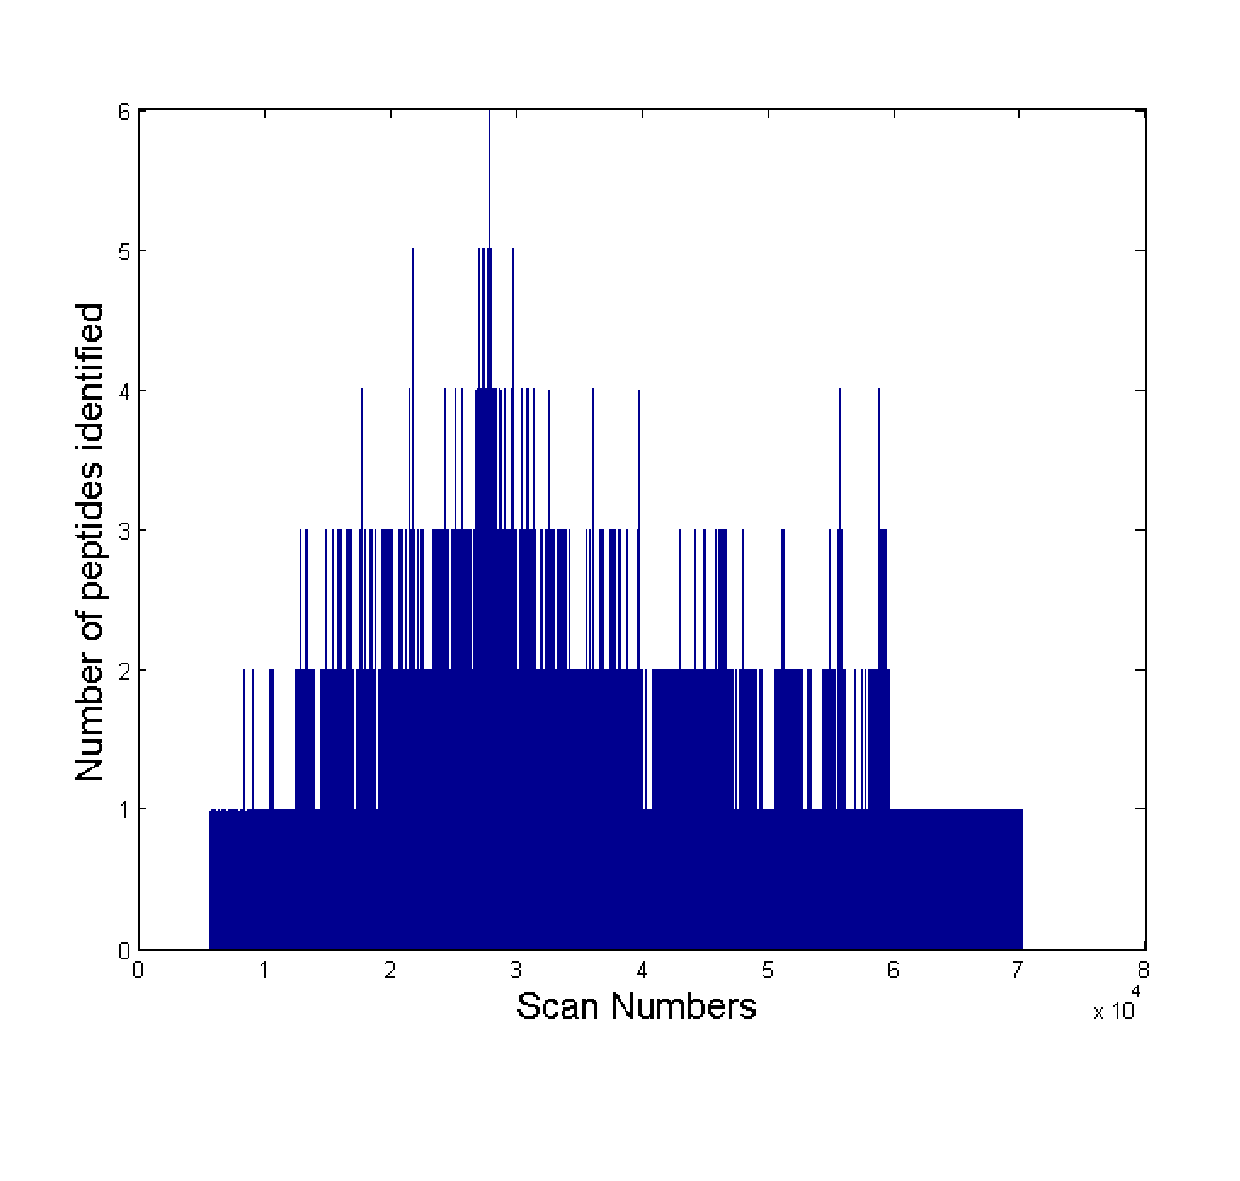
\includegraphics[height=75mm, width=100mm]{./Figures/swath_pepcounts}
\caption{\footnotesize {\bf Peptide identification of SWATH data.} We searched each SWATH spectrum against all candidates in the spectral library that are within the precursor mass tolerance.  Matches were sorted according by their projected-cosine score and a 1\% FDR was enforced using the TDA approach.  For the UPS1+ E. Coli dataset we counted the number of matches for each SWATH spectrum.  In many cases we identify multiplexed spectra (with two to six peptides).
% indicating the feasibility of identifying multiplexed spectra in DIA workflows using spectral library search.
}
\label{Swath_pep_counts}
\end{figure}
	
\subsubsection{Identification of multiplexed spectra using linear programming}

%M-SPLIT models an observed multiplexed spectrum as a linear combination of two single-peptide spectra: $M=A+\alpha B$. The %multiplexed spectrum is then identified by finding the pair of
%single-peptide
%spectra in a library $\mathcal{L}$ that best matches the multiplexed spectrum.  To remove any assumptions regarding the %number of peptides present in the multiplexed spectrum,

We now propose to generalize M-SPLIT  to model a multiplexed spectrum as a linear combination of \emph{all} spectra in the library: $M \approx \sum_{i=1}^{|\mathcal{L}|}{\alpha_{i}S^{i}}$ where $S^{i}\in \mathcal{L}$ and $mass(S^i)$ is within tolerance of $mass(M)$.  Since the $\alpha_i$ mixture coefficients model the relative abundances of co-fragmented peptides, those that are not present in the multiplexed spectrum should result in corresponding $\alpha_i\approx 0$. Using this formulation, we can apply linear programming (LP) techniques to find a subset of
%single-peptide
library spectra that best matches a given multiplexed spectrum. Specifically, let $M = m_{1}, m_{2}, ... m_{n}$ be a multiplexed spectrum and $S^{j} = {s^{j}_{1}, s^{j}_{2}, ..., s^{j}_{n}}$ be the $j^{th}$
%single-peptide
spectrum in a library $\mathcal{L}$.
%We then define the following relationship:
Since $m_j \approx \sum_{i=1}^{|\mathcal{L}|}  \alpha_i \times {s^{i}_j}$, we can model the error for each peak as follows

\[
\epsilon_j = m_j - \sum_{i=1}^{|\mathcal{L}|} \alpha_i \times{s^{i}_j}
\]

The following problem with non-negative variables $\alpha_1, \ldots , \alpha_{|\mathcal{L}|}$
 minimizes the sum of absolute values of errors for each peak. While the objective function is non-linear, it can be easily reduced to the standard linear program (LP) by introducing additional variables.
%We then generate an LP instance which minimizes the error of each peak:

\[
\begin{array}{l|l|l}
{\rm Input} & {\rm Output} & {\rm Formulation} \\
\hline
\begin{array}{l}
s^{i}_j \mbox{ for every  } i, j \\
m_j \mbox{ for every  } j \\
\end{array}&
\begin{array}{l} \alpha_i \mbox{ for every spectrum}\\
                      \mbox{ in the library $\mathcal{L}$ }
\end{array}&
\begin{array}{cll}
\min &{\displaystyle \sum_{j=1}^{n}{|\varepsilon_j|}}\\[1.5em]
%{\rm s.t.} & \sum_{p_j\in P} Q_i = 100 & \\[1.5em]
{\rm s.t.}&{\displaystyle \varepsilon_j = m_j - \sum_{i=1}^{|\mathcal{L}|} s^{i}_j \times{\alpha_i} }\\
[1.5em]
&{\displaystyle \alpha_i\geq 0} \\
\end{array}\\
&&\\
%&&\alpha_is\mbox{ are normalized prior to output so that } \sum_i(\alpha_i) = 1\\
\end{array}\\
\]

%Essentially, the LP estimates how much each candidate peptide contributes to the abundance of each peak in $M$ %based on the weighted summed intensities of the matching peaks in the single-peptide spectra. It then minimizes the %resulting error by comparing these predicted intensities to those in $M$.
Intuitively, in the solution of the resulting LP, a higher $\alpha_{j}$ for a  spectrum $S^{j}$ corresponds to a more significant match between the multiplexed spectrum $M$ and $S^{j}$.  In the extreme case where $\alpha_j=1$, the candidate spectrum $S^{j}$ is a ``perfect'' match to $M$.  Therefore we can use the resulting $\alpha$ as scores for each of the matches between multiplexed and library spectra and enforce FDR by adapting the TDA approach for spectral library searches~\cite{lamdecoylib}.

{\bf Identification of multiplexed spectra from modified peptide variants.} To demonstrate the feasibility of the LP approach we tested it in the context of determining site assignments of PTMs. While identification of modified peptides is appropriately controlled by FDR~\cite{beausoleil04,Trinidad2012}, the lack of an equivalent approach for {\em PTM site assignments} often results in the need for extensive manual validation. Probabilistic scoring methods such as AScore~\cite{beausoleil06} have begun to address this need, but still do not offer a global, data dependent measure of the quality of localization results. %To date the recommended fixed thresholds for site assignment are mostly based upon the empirical false localization rates estimated from specific small sets of synthetic peptides rather than re-estimated for each experiment. Moreover, since fixed thresholds may correspond to varying FLRs on different data, these also do not offer a way to compare competing fixed threshold scoring methods of the same datasets.

We propose a new framework for estimating  false discovery rates for PTM site assignments that we refer to as  {\em False Localization Rates (FLRs)}.   First, our approach assigns scores to PTM {\em variants} of the same peptide, where each variant is a different combination of site assignments for the same PTMs on the same peptide sequence. Second, we extend the concept of the Target-Decoy Approach~\cite{Elias2007}
%where invalid peptide sequences are used to estimate false identification rates against valid peptide sequences
and use invalid (decoy) PTM site assignments, such as phosphorylation on Glycine, to estimate FLR on valid (target) sites. Third, we allow each spectrum to be composed of more than one variant, thus allowing for identification of  $i$) ambiguous PTM site assignments (i.e., indistinguishable variants due to incomplete MS/MS fragmentation) and $ii$) multiplexed spectra from co-eluting peptide variants, %s with the same modification on the same peptide sequence but with different modification sites,
thus possibly resulting in multiple correct site assignments per spectrum (e.g., as in histones~\cite{DiMaggio2009}).

The proposed approach models a spectrum as a linear combination of spectra from all possible PTM variants and assigns a separate score to each distinct variant. The spectrum for a particular PTM variant is predicted from the spectrum of the unmodified peptide by shifting ions from their unmodified fragment masses to their corresponding theoretical masses for modified fragments.  Ambiguity is addressed by grouping indistinguishable variants (i.e., with no distinguishing ions between modification sites) into {\em variant groups} and co-elution is automatically captured by co-occurrence of high-scoring distinct variants in the same  spectrum. An overview of this approach is illustrated in Figure~\ref{fig:flowchart}.

%\begin{landscape}
%\begin{figure}
\begin{sidewaysfigure}
%\centering % trim=l b r t
\begin{center}
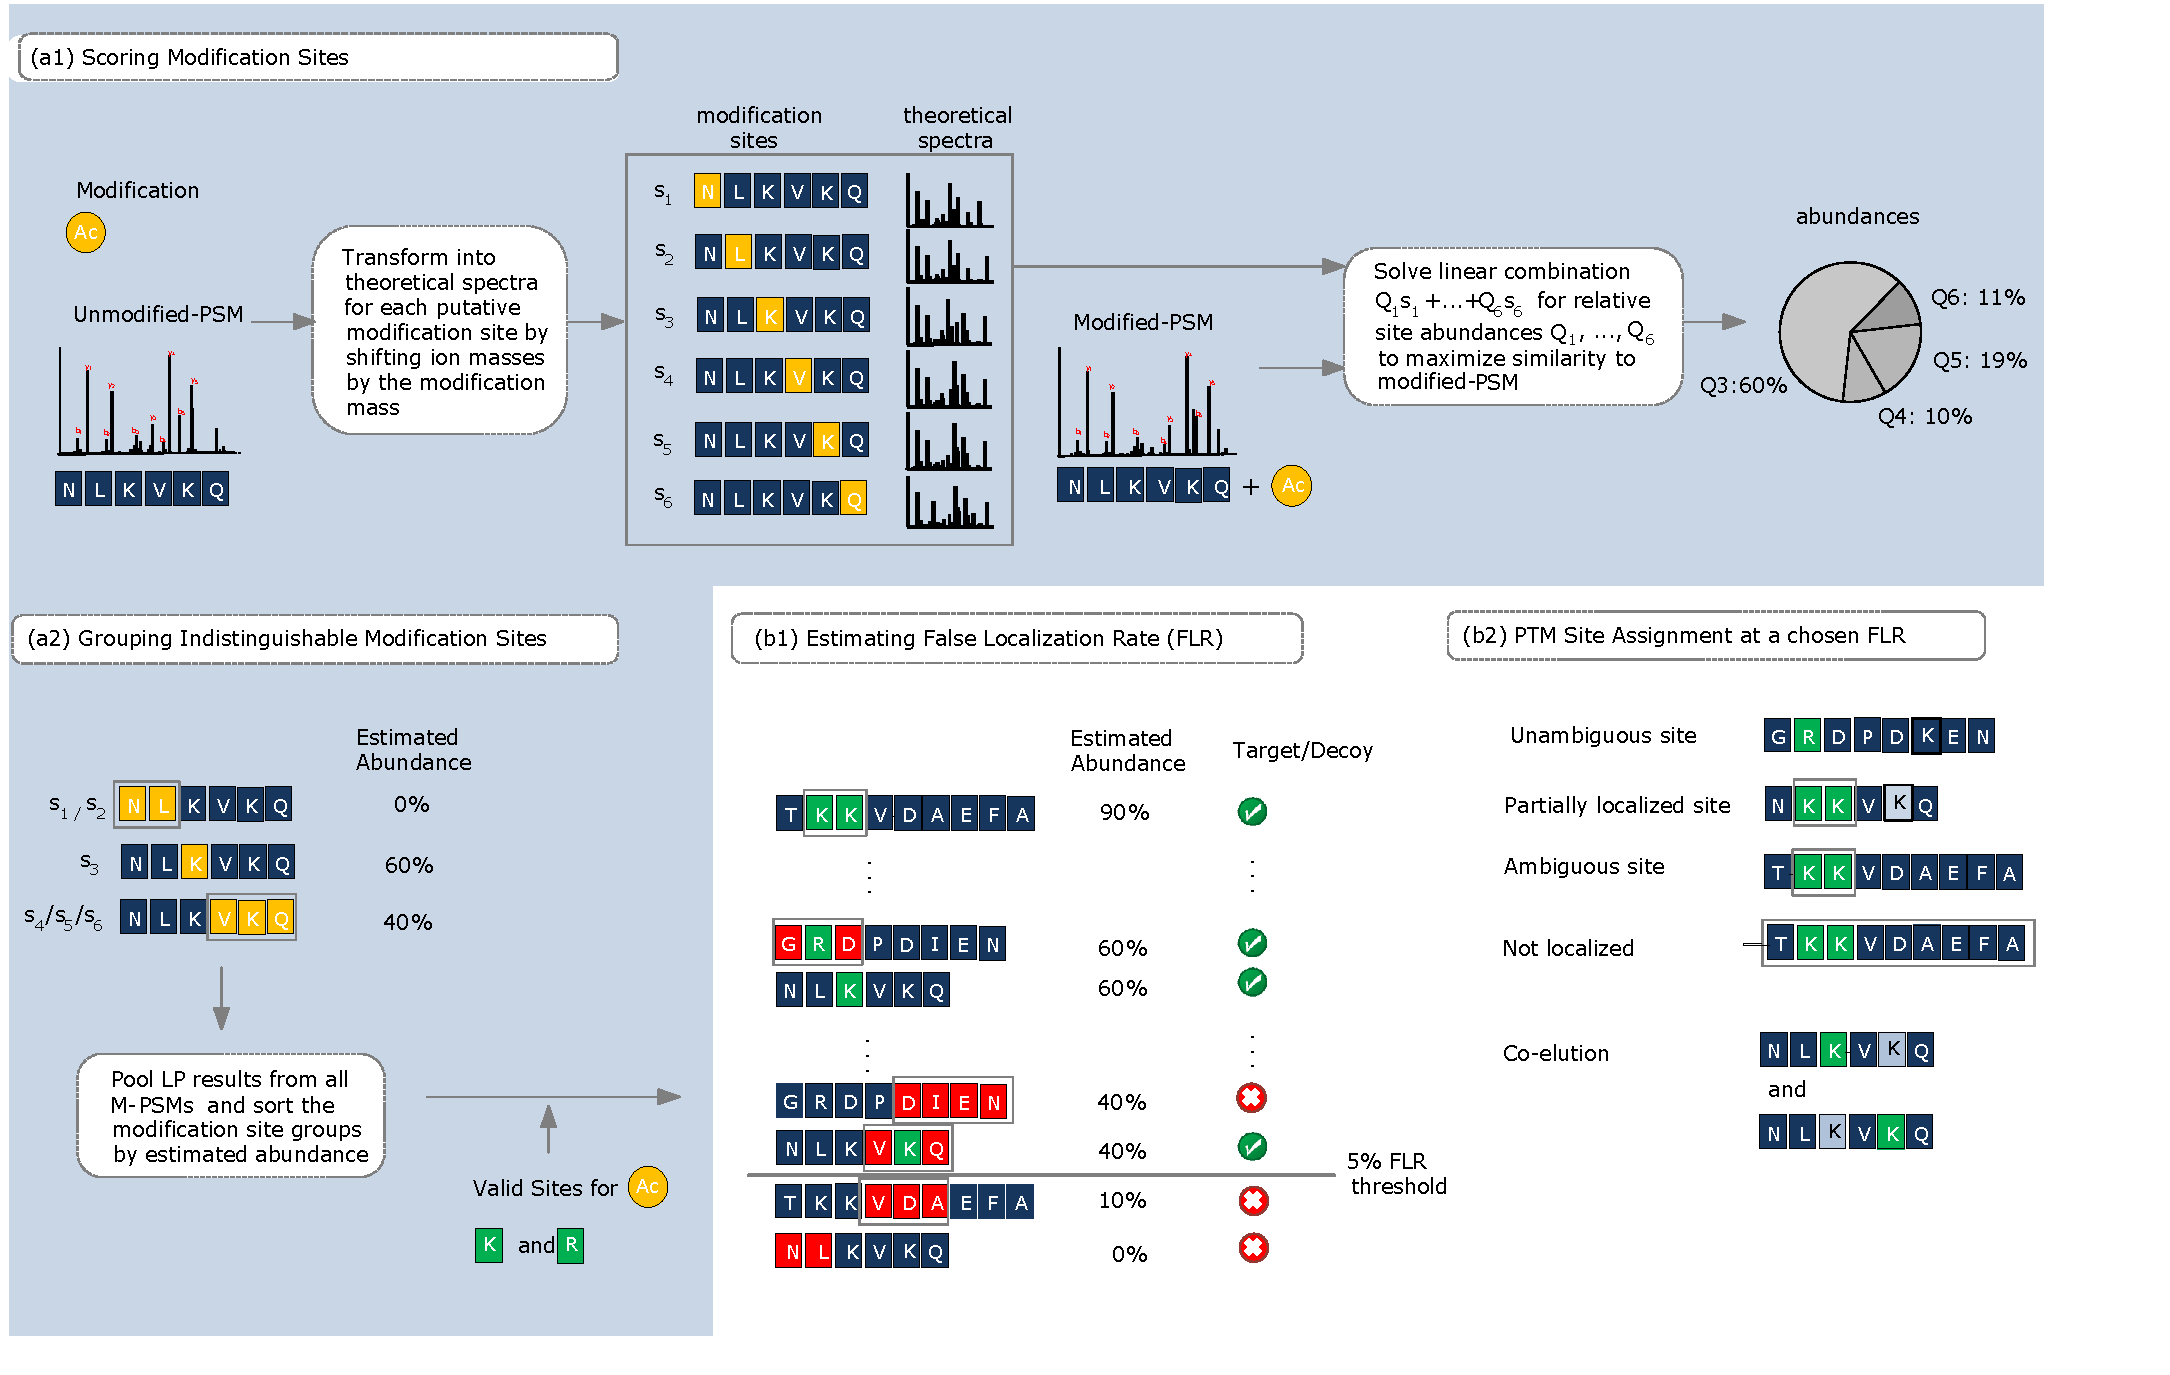
\includegraphics[height=120mm]{./Figures/FLR/intro}
\caption{\footnotesize {\bf Overview of the FLR approach.} %a) all modification sites are scored individually. b) invalid site assignments are used as decoys for TDA-like calculation of FLR. (a1) For each modified spectra, the first step in PTM localization is to score each putative modification site.
(a1) Using predicted spectra for each peptide {\em variant} with the same PTMs on different sites, we model each observed spectrum as a linear combination of all possible variants and use linear programming to determine the relative abundance (i.e., mixture coefficients) for each variant.
% This is done by taking the ion intensities (bs and ys for CID) from an unmodified spectra of the same peptide and assuming that the associated ions in the modified spectrum will be the same. The intensities are shifted by the correct masses based on the particular modification site to generate a theoretical spectra for each possible modification site. An LP is then formulated which calculates the quantity of each modification site based on the overall contribution of each theoretical spectra to actual modified spectra.
(a2) Ambiguities in site assignment caused by incomplete MS/MS fragmentation are handled by grouping indistinguishable variants into groups. %Due to the missing peaks in the modified peptide spectrum, some modification sites are indistinguishable to the LP.
In such cases, we report the coefficients for the variant groups instead of the those of the individual variants.
(b1) A TDA strategy is adopted to determine the global false-localization rate (FLR) for site assignments. The knowledge of the PTM site-specificity is introduced at this point: variants or groups assigning the PTM to at least one valid site are considered target matches. Conversely, variants or groups that assign the PTM to invalid sites only are considered decoy matches. % Once the target and decoy site assignments are made, each site group is scored by the total estimated abundance.
Variant groups are then ranked by decreasing mixture coefficients and FLR is calculated at each threshold by the ratio of target/decoy site assignments.
(b2) PTM site assignments at a chosen FLR are reported. If the peptide has one reported group with one valid site only, then the modification is unambiguously assigned to that valid site. If the reported group has more than one possible valid site but excludes other valid sites, then it is considered partially localized. If the reported group has multiple valid sites, then the site assignment is ambiguous. If the reported group contains all possible variants then it is considered a non-localized result. Multiple groups passing the score threshold for the same peptide are an indication of co-elution of PTM variants.% where the relative scores can be interpreted as the relative abundances of the co-eluting sites.
\label{fig:flowchart}}

\end{center}
\end{sidewaysfigure}
%\end{figure}
%\end{landscape}

We evaluate the performance of our FLR approach on phosphorylation site assignment. In brief, {\em S. Cerevisiae} lysates were IMAC-enriched for phosphopeptides and MS/MS spectra and neutral-loss dependent MS/MS/MS spectra were acquired using an LTQ Orbitrap XL. %from the first half of the sample. The second half of the sample was CIP treated for removal of the phosphate group, HILIC fractionated into 11 fractions and MS/MS were acquired on the de-phosphorylated peptides.
%
All spectra were searched using InsPecT~\cite{tanner05} at 1\% FDR. %with parent mass tolerance $2$ Da and fragment mass tolerance $0.5$ at $1\%$ spectrum false discovery rate.
Spectra identified as modified peptides were then processed by FLR and Ascore~\cite{beausoleil06} to perform site assignments.  Figure~\ref{AScoreLPCompare} shows the number of results at an FLR of $5\%$ and the equivalent AScore threshold of 13. Although the overlap between Ascore and FLR is very high, FLR was able to confidently assign PTM sites in significantly more MS/MS and MS/MS/MS spectra.

\begin{figure}[h!]
\centering
\vspace{-0.9in}
%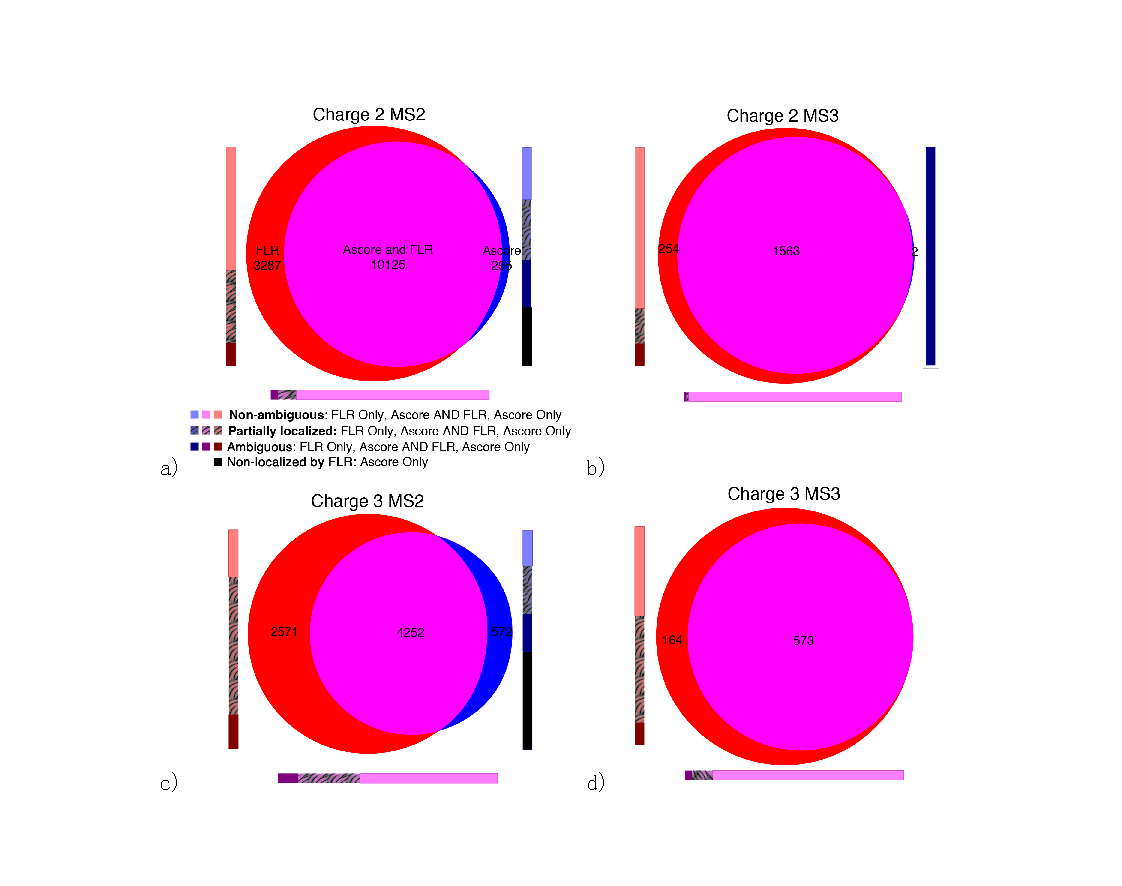
\includegraphics[height=150mm, width=132mm]{./Figures/FLR/FLR_yeast_phosovenn}
%\scalebox{1.0}{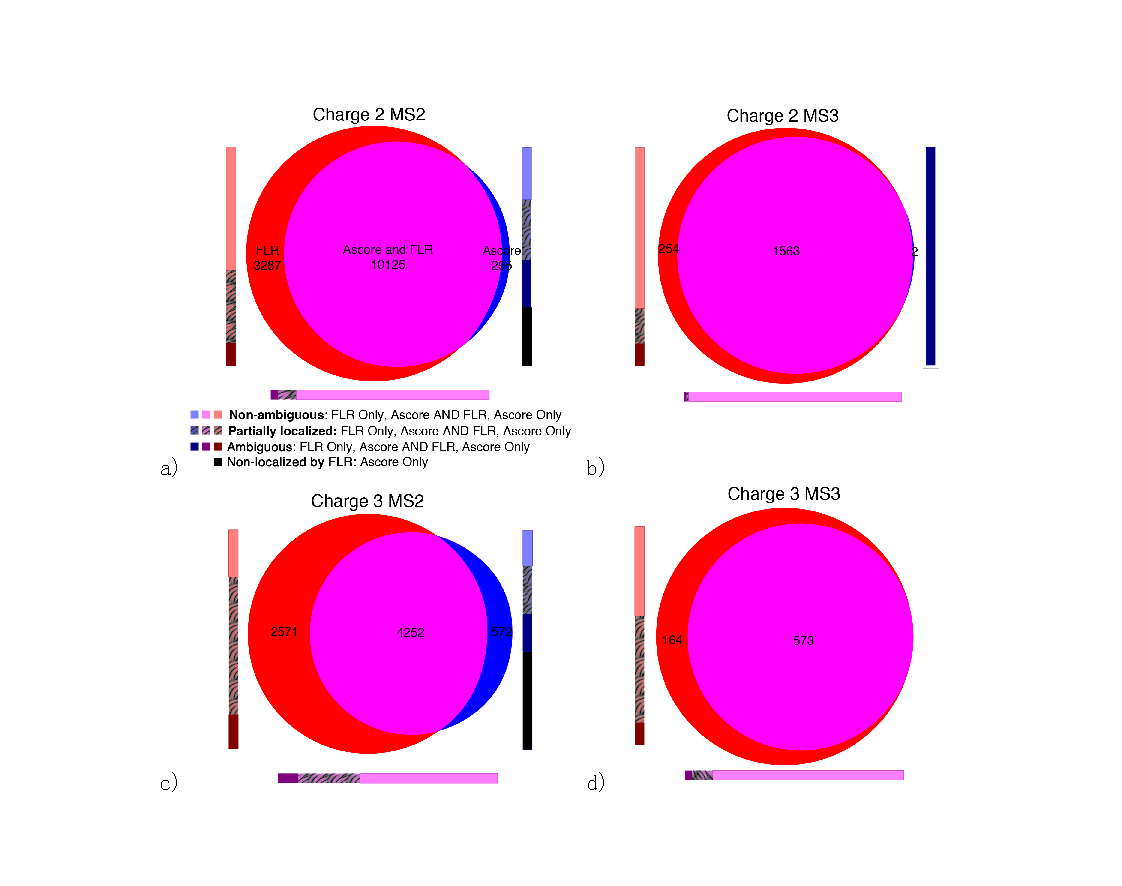
\includegraphics[trim =10mm 0mm 0mm 0mm, clip, width=7in]{./Figures/FLR/FLR_yeast_phosovenn}}
\scalebox{1.0}{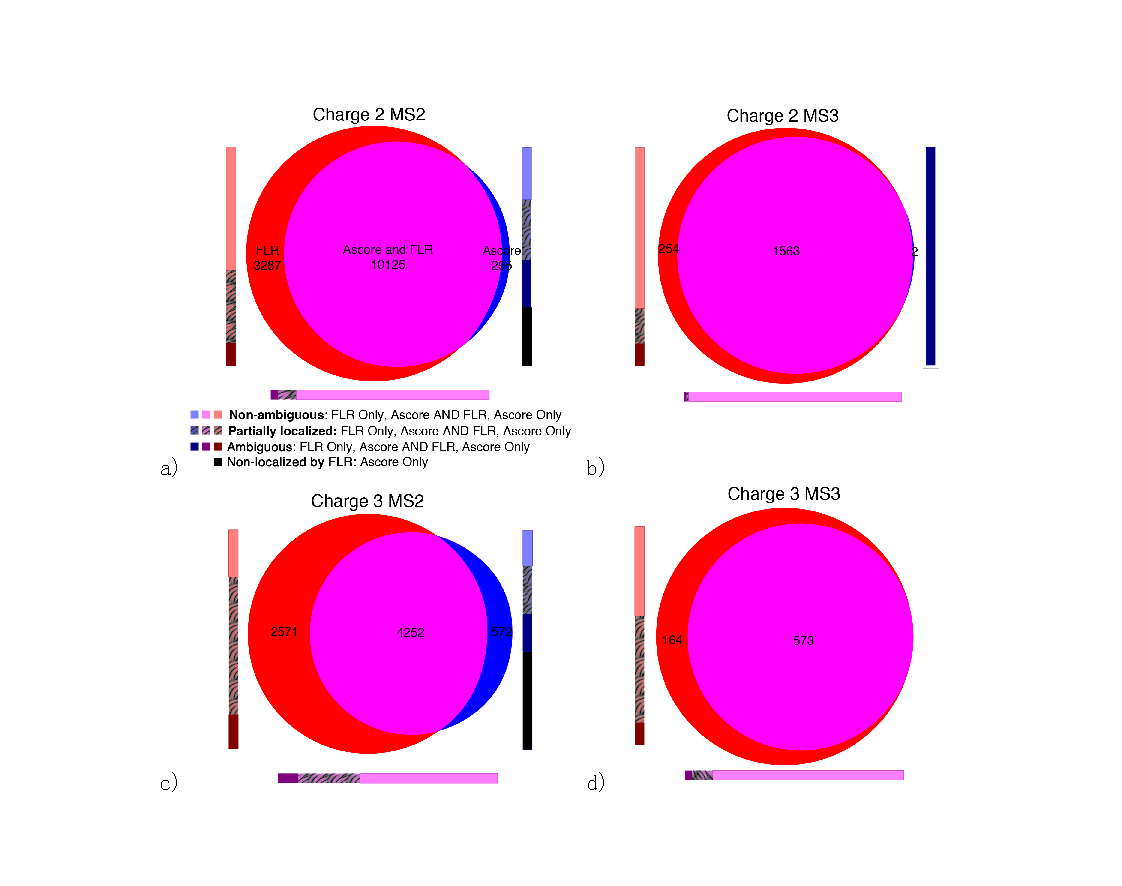
\includegraphics[trim =10mm 0mm 0mm 0mm, clip, width=7in]{./Figures/FLR/FLR_yeast_phosovenn}}
\vspace{-0.9in}
\caption{\footnotesize {\bf Ascore vs. our False Localization Rate (FLR) approach for phosphorylation results.} {\em Non-ambiguous} are FLR results returning only one valid variant. {\em Partially localized} results exclude possible valid sites but still cannot distinguish between more than one valid variant. {\em Ambiguous} does not exclude any valid site but still excludes incorrect variant sites. {\em Non-localized} means that all possible variants are in one group, no valid or invalid sites are excluded. Non-localized results are included as Ascore-only as FLR does not return any localization information. An FLR cutoff of .05 and an Ascore cutoff of 13 was used. a) Charge 2 MS2 results out of $14,127$ identified by InsPecT. $13,412$ passed the FLR cutoff, $10,420$ passed the Ascore cutoff. b) Charge 2 MS3 results out of $1,898$ identified by InsPecT. $1,817$ results passed the FLR cutoff, $1,565$ results passed the Ascore cutoff. c) Charge 3 MS2 results out of $7,897$ InsPecT results. $6,823$ passed the FLR cutoff, $4,824$ passed the Ascore cutoff. d) Charge 3 MS3 results out of $803$ Inspect results. $737$ results passed the FLR cutoff, $573$ passed the Ascore cutoff.}
\label{AScoreLPCompare}
\end{figure}

{\bf Improving the LP formulation with filtration.}
%While the LP formulation proposed above
%(i.e., $M=\sum_{i=1}^{|\mathcal{L}|}{\alpha_{i}S^{i}}$ where $S^{i}\in \mathcal{L}$)
% is conceptually straightforward,
The optimal solution of the LP problem above does not necessarily correspond to the correct peptides co-fragmented in the multiplexed spectrum. Considering {\em all} spectra in the spectral library  $\mathcal{L}$ may (i) make the LP instance too large resulting in a slow algorithm, and (ii) incur a high risk of false-positive identifications if some spectra can be decomposed as linear combinations of other library spectra.
%
% If every spectrum in the library is allowed in the LP formulation then it would be inefficient to solve such large LP %instances and there would be a higher risk of false-positive identifications if some spectra can be decomposed as linear %combinations of other library spectra.
This is not an issue for FLR because there is only a small number of PTM variants and thus the ``spectral library'' is very small. Therefore for  identification of multiplexed spectra we will first filter the spectral library to a small subset of promising candidates and then apply the LP formulation only on this reduced subset.  M-SPLIT results show that projected-cosines are an efficient filter  reducing the search space by orders of magnitude. Several other filters can also be used to further improve filtering efficiency. For example peptide sequence tags have been used extensively in database search tools to reduce the effective size of the sequence database, but this approach has not yet been applied to spectral library searches. % A similar strategy can also be applied to spectral library searches since these can also be seen a reduced database containing only sequences for previously-identified peptides.
Another route towards improving filtration efficiency is based on the observation that while cosine is a good measure for spectral similarity, it is not well normalized across different types of
s. For example, low complexity spectra tend to be dominated by a few high intensity peaks (e.g. spectra from proline-containing peptides) and often result in artificially high projected-cosine scores by matching only one or two peaks. % Therefore it is expected that many candidate peptide spectra passing the projected-cosine filter are not really present in the multiplexed spectrum.
We propose to address this issue by simply adding the requirement that the $K$ highest-intensity fragment ion peaks in a library  spectrum must be present in the multiplexed spectrum. The values of $K$ resulting in the best filtration efficiency will be learned  from data for different types of peptides (e.g., unmodified vs phosphorylated) and MS/MS fragmentation modes (e.g., CID, HCD, ETD).

%Finally we note that when multiple LP solutions are equally good, one would probably prefer solutions that involve lower numbers of peptide candidates from the spectral library.  Intuitively, an identification of a multiplexed spectrum is more believable if 2 peptides explain the observed spectrum than if otherwise 10 peptides are needed to explain the observed spectrum equally well.  When more peptides are involved it is statistically more likely that false positive identifications can result just by random chance.  To address this, we will introduce regularization terms~\cite{han1979exact} in the LP objective function that penalize for the number of candidate spectra in the final LP solution. For example, the objective function in the LP can be modified as follows: $\min {\displaystyle \sum_{j=1}^{r}{|\varepsilon_j|} + \sum_{i=1}^{|\mathcal{L}|}{\delta\alpha_{i}}}$, where $\delta$ is a nonnegative regularization parameter.

{\bf Extending the LP formulation for DIA LC/MS/MS maps.}
The above LP formulation models each multiplexed spectrum as an independent entity.  However, one of the most informative features of DIA is that the same peptides are observed across multiple MS/MS spectra throughout their elution profile.  The resulting correlation between DIA spectra containing the same peptides has been shown to reduce noise~\cite{blackburn2010}, allow grouping peaks from the same peptides across multiplexed spectra~\cite{blackburn2010,bern2009}, and enable peptide quantification~\cite{Gillet12targeted}.

Since DIA spectra can only contain fragments from the same peptides whenever the corresponding survey scans contain precursor peaks from the same peptides, we will start our analysis of LC/MS/MS maps by first using feature detection software such as MaxQuant~\cite{cox2008maxquant} or OpenMS~\cite{sturm2008openms} to find all LC/MS peptide features.  These will then be divided into non-overlapping groups according to their retention time and m/z.  First we will divide the features into groups by their m/z values according to the MS/MS isolation window of the DIA method.  Features from different isolation windows are fragmented in unrelated multiplexed spectra and thus do not need to be considered together.  Next we will separate features within the same isolation window by grouping features whose elution profiles overlap in retention time.  An example of how to group MS features on an LC/MS map is illustrated in Figure~\ref{multi_LP_2D}a, where the features are separated into three groups.

Once features are divided into groups,  we propose to model {\em sets} of related DIA MS/MS spectra by extending our LP formulation.
%To take advantage of such correlated DIA spectra for peptide identification, we propose to extend our LP formulation to {\em sets} of multiplexed spectra.
%
To illustrate this idea, imagine a simple example where there are only two peptides $A$ and $B$ in each of two multiplexed spectra $M_{1}$/$M_{2}$ acquired at elution times $T=1,2$, respectively (see Figure~\ref{multi_LP_2D}b); peptide $A$ ($B$) is observed with precursor abundance $\alpha_{A1},\alpha_{A2}$ ($\alpha_{B1},\alpha_{B2}$) at $T=1,2$ (estimated from MS1 survey scans). Finally, we have a spectral library $\mathcal{L}=\{P,Q,R\}$ that contains only three candidate spectra where $P$ and $R$ have the same precursor mass as peptide $A$ and $Q$ has the same precursor mass as peptide $B$.

Intuitively, we are trying to find a subset of candidates in $\mathcal{L}$ that best match both $M_{1}$ and $M_{2}$.  We start by defining an LP objective function for each $M_{j}$ as before (see Step 1 in Figure~\ref{multi_LP_2D} c).  Next we impose a relationship between the LP solutions across the two neighboring multiplexed spectra.  % Let $\alpha_{A1}$ be the true relative abundance of peptide feature $A$ in $M_{1}$ as estimated in the corresponding MS1 survey scan (see Figure~\ref{multi_LP_2D}b).
Let $\alpha_{P1}$ and $\alpha_{P2}$ be the relative abundances estimated by LP for peptide $P$ in $M_{1}$ and $M_{2}$, respectively. The key idea that we introduce here is that if $A$ and $P$ are the same peptide then the LP-estimated abundances for $P$ (i.e., $\alpha_{P1}, \alpha_{P2}$) should match the MS1-derived abundances (i.e., $\alpha_{A1}, \alpha_{A2}$), such that $\frac{\alpha_{P1}}{\alpha_{A1}} \approx \frac{\alpha_{P2}}{\alpha_{A2}}$.
% the we should we expect in the correct LP solution $\frac{\alpha_{P1}}{\alpha_{A1}} \approx \frac{\alpha_{P2}}{\alpha_{A2}} \approx 1$. Similarly if $Q$ and $B$ are the same peptide  $\frac{\alpha_{Q1}}{\alpha_{B1}} \approx \frac{\alpha_{Q2}}{\alpha_{B2}}\approx 1$.
Similarly if $Q$ and $B$ are the same peptide then $\frac{\alpha_{Q1}}{\alpha_{B1}} \approx \frac{\alpha_{Q2}}{\alpha_{B2}}$. This is implemented in the LP by adding new error terms for candidate P: $\delta_{P12} = |\frac{\alpha_{P1}}{\alpha_{A1}} - \frac{\alpha_{P2}}{\alpha_{A2}}|$ and similar error terms for every other candidate from the library (step 2 in Figure~\ref{multi_LP_2D}c).
%To implement this idea in LP we can define a new objective function for candidate $P$: $\delta_{P12} = \frac{\alpha_{P1}}{\alpha_{A1}} - \frac{\alpha_{P2}}{\alpha_{A2}}$. The same cost function can be defined for each candidate in the library(see step 2 in Figure~\ref{multi_LP_2D}c).  The quantity $\delta$ should be close to zero if LP select the correct candidates in the library for both multiplexed spectra.  This new cost function serves two purpose.
%
These new error terms serve two purposes. First, they promote agreement between the relative abundances in the LP solution and the estimates from MS1 survey scans, thus integrating information from both MS and MS/MS spectra. Second, they impose consistency between LP solutions for consecutive multiplexed spectra $M_{1}$ and $M_{2}$.
%
To illustrate this point, consider a situation where LP selects candidates $P$ and $Q$ for $M_{1}$ and finds two equally good solutions for $M_{2}$: one selecting $P$ and $Q$ and another selecting $P$ and $R$. With the new error terms, LP will prefer a solution where the same set of candidates ($P$ and $Q$ in this case) are selected for both multiplexed spectra.
%This way information from both spectra are used in synergy for peptide identification.
This is a strong constraint since we expect information in multiple DIA MS/MS spectra to be correlated but also somewhat different.

In contrast to DDA workflows, consecutive DIA MS/MS spectra are not mere re-acquisition of the same peptides. Distinct peptides tend to co-elute at unrelated abundances in close elution times (e.g., different slopes in the elution curve) and thus the DIA MS/MS interference between these peptides is also likely to change. As a result, different time points may reveal different subsets of DIA MS/MS fragment ions of a particular peptide that are free of interference. Integrating such information across multiple DIA MS/MS spectra is thus likely to both decrease false positive identifications (by promoting consistency) and also increase the sensitivity of peptide identifications (by aggregating more abundance in the correct peptides instead of splitting it across linearly dependent sets of peptides).

\begin{figure}[h!]
	\centering
		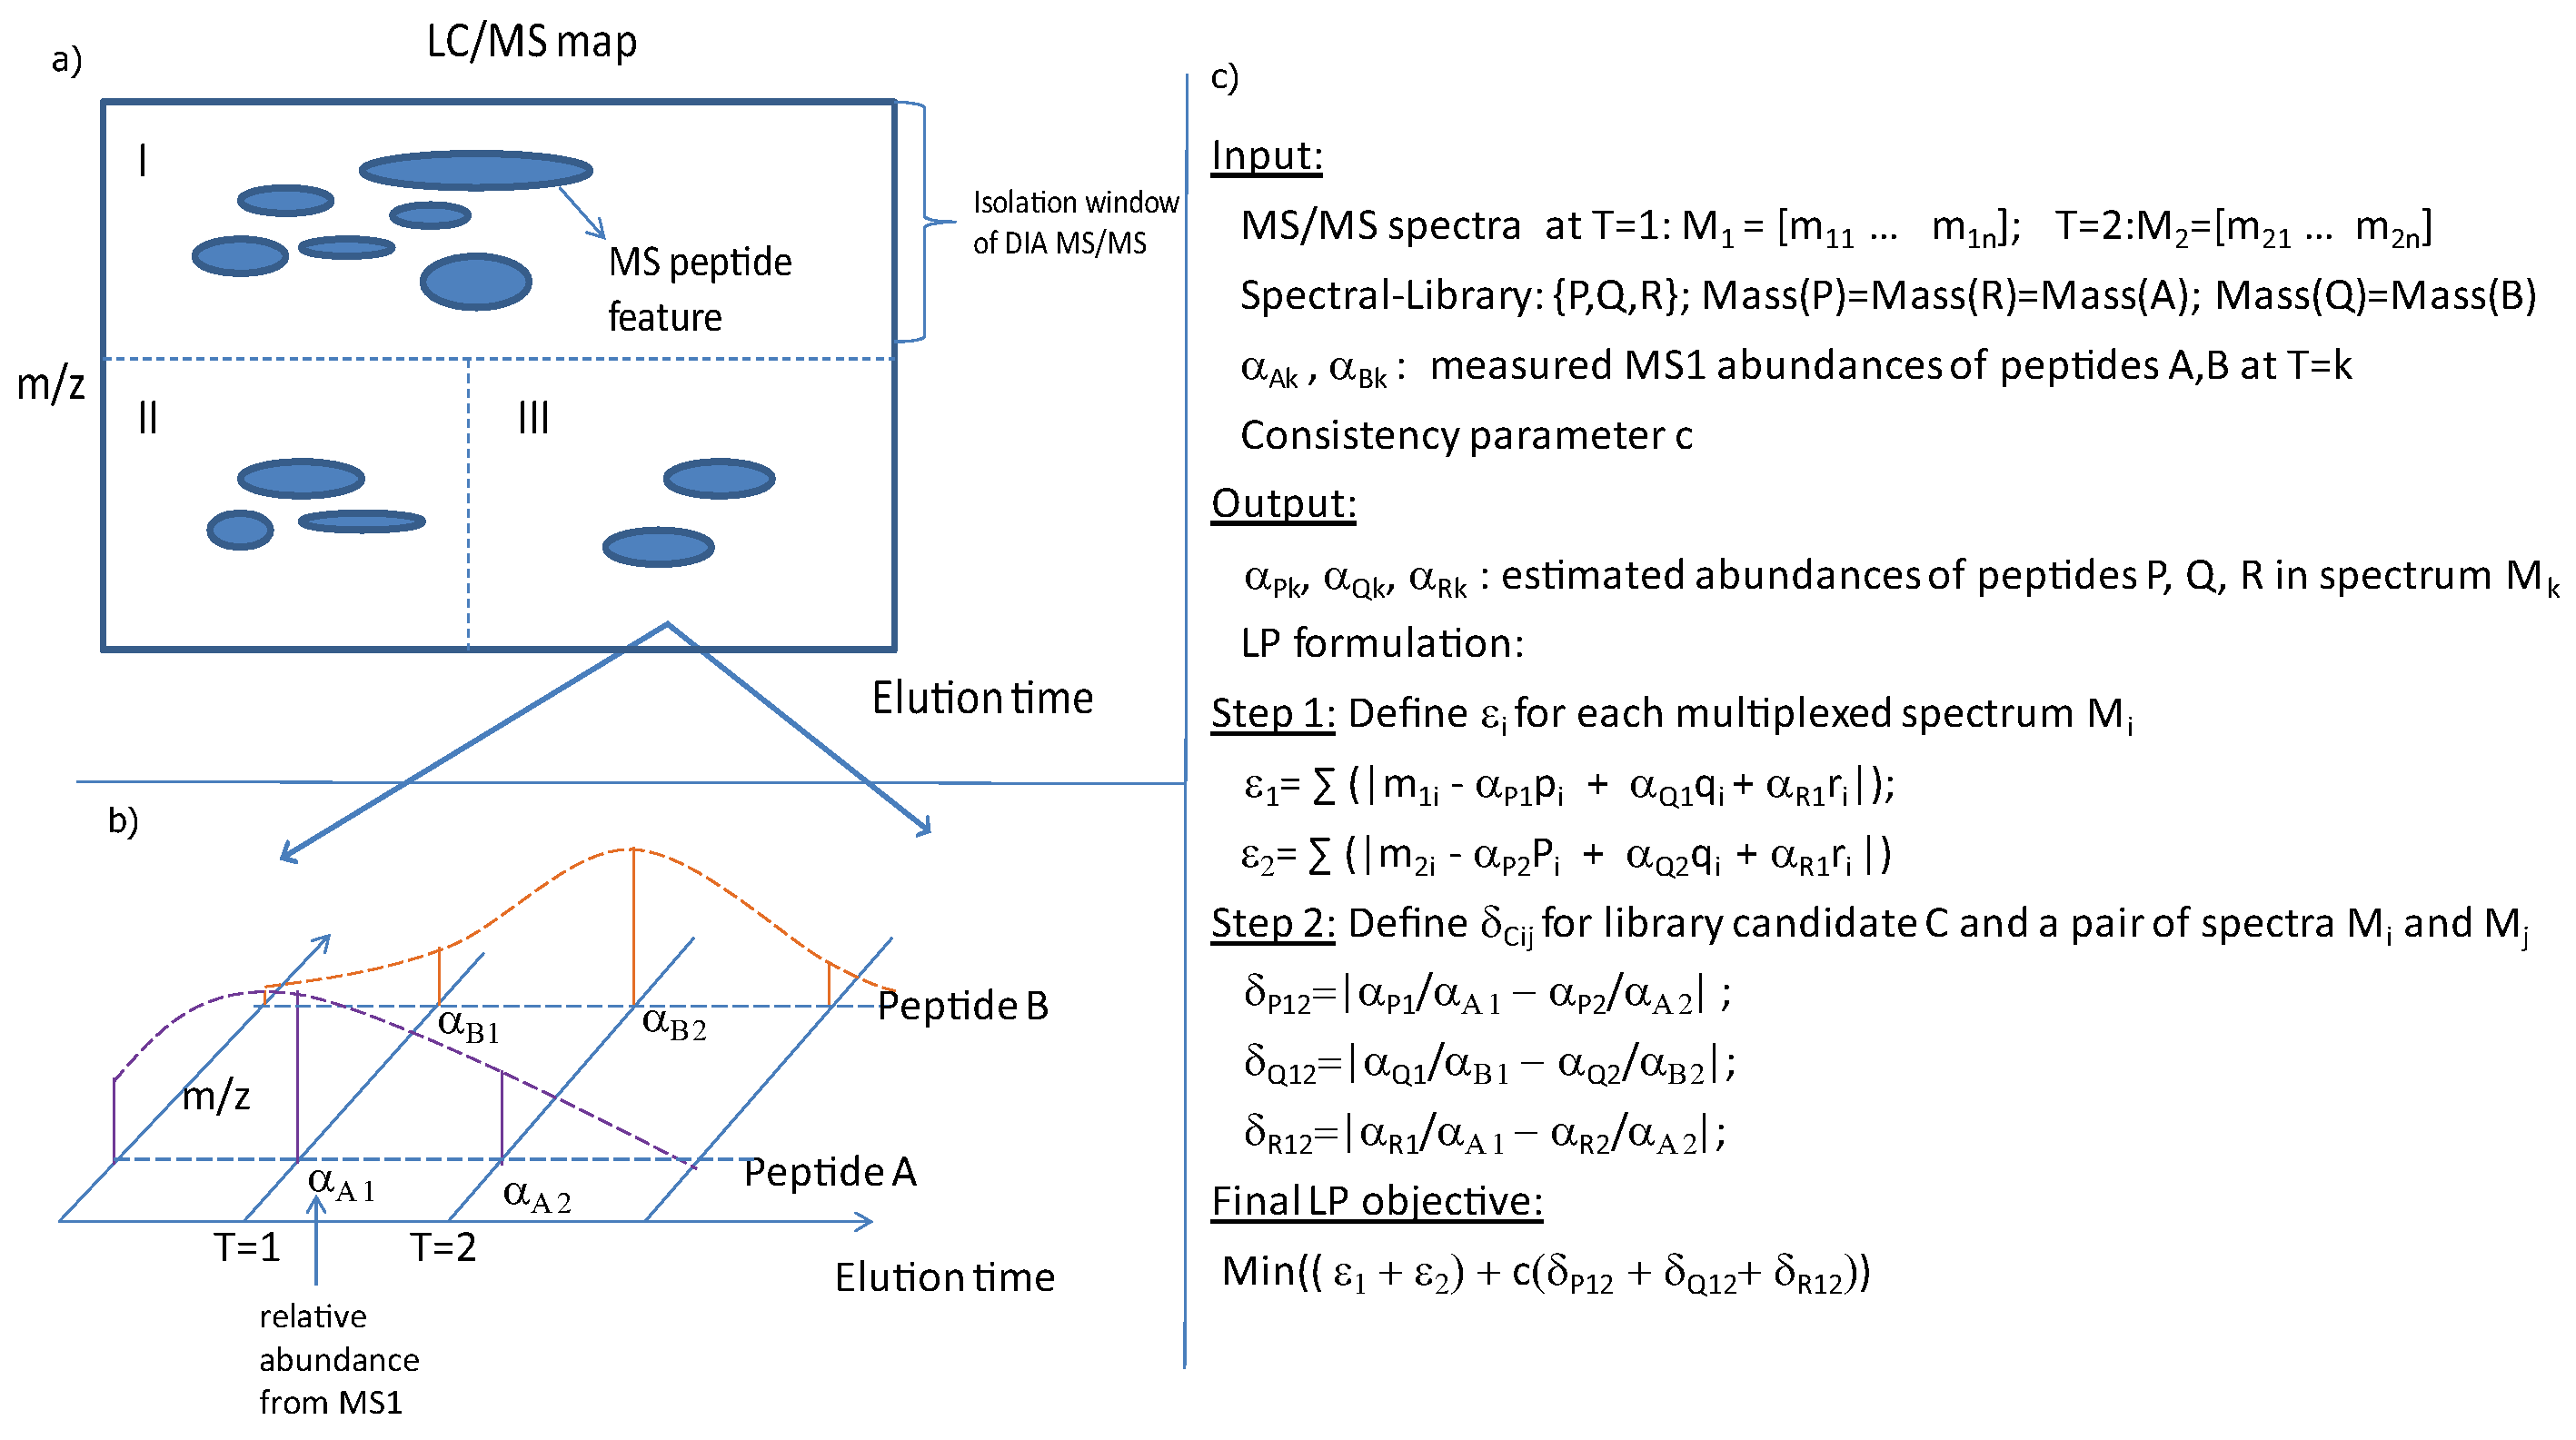
\includegraphics[height=90mm, width=165mm]{./Figures/Multiplexed_2D_LP}
		\caption{\footnotesize {\bf LP formulation for DIA LC/MS/MS maps.} a) To reduce the complexity of the problem we divide the LC/MS map into separate regions with no overlapping peptide features. The LC/MS map is first divided along the m/z axis according to the isolation window of the DIA method. Since peptides in different isolation windows do not fragment in the same multiplexed spectrum they are not considered together.  Next, within the each isolation window, peptide features overlapping in retention time are grouped together. Each resulting group of features corresponds to a distinct region on the LC/MS map. We formulate an LP instance for each region.  The example in a) divides the LC/MS map into three regions.  b) A simple scenario where a region contains only two peptides $A$ and $B$ is illustrated. $\alpha_{Ak}$/$\alpha_{Bk}$ indicate the relative abundances peptides $A$/$B$ (respectively) at time $T=k$ as estimated by the peak intensity in the corresponding MS1 survey scans. Two multiplexed spectra are acquired that contain both $A$ and $B$. c) The LP formulation for the region in b) is illustrated.}
	\label{multi_LP_2D}
\end{figure}

To generalize from this simple two-spectrum case to a set of consecutive multiplexed spectra $\{M_{1} ... M_{k}\}$ (for the same precursor isolation window), we note that the $\epsilon_{i}$ terms are defined for each multiplexed spectrum and can thus be easily generalized to a set of spectra. The $\delta$ terms are defined per peptide candidate and per pair of multiplexed spectra. For each peptide and a set of spectra, we can either define a $\delta$ term for every consecutive pair of spectra (linear consistency penalty) or for all possible pairs of spectra (quadratic consistency penalty). % This will determine how consistent we want the LP solutions across different spectra to be. An more adaptive solution will be to define a window $W_{i}$ that spans the elution profile of the candidate and create a $\delta$ term for the candidate only within that window.

%\subsubsection*{future extensions}
%\begin{itemize}
%    \item Extending LP model for multiplexed spectra: determine abundance coefficients for each peptide and use those as scores for FDR calculations
%    \item Improving filtration to reduce number of spectra used for LP: e.g., sequence tags, rank order or cosine with top 5 peaks in the library or top k out of n
%    \item Extending LP model for 2D matches with DIA LC/MS/MS
%\end{itemize}

\subsection{Aim 2: Database search of multiplexed spectra}

Despite the rapid growth of spectral libraries, methods based on spectral matching suffer from the limitation that peptides cannot be identified if they have not been observed before. Moreover, while spectral libraries from CID fragmentation are quite comprehensive, spectral libraries from other fragmentation methods (e.g. ETD, HCD) are still limited. Hence database search remains the dominant approach for peptide identification.  Some database search tools approach the multiplexed spectra identification problem by reporting spectra with more than one significant single-peptide match and do not explicitly attempt to models the occurrence of fragment ions from two peptides in the same spectrum.  False Discovery Rates (FDR) are also left unadjusted \cite{zhang2005tree} and may result in higher than expected FDR for second IDs (e.g., when co-eluting peptides share a substantial number of fragment masses). In difference from previous approaches, our  MixDB~\cite{wang2011peptide} database search tool for multiplexed spectra uses a scoring model specifically designed for matching spectra against more than one peptide and determines separate FDRs for identification of single-peptide spectra and multiplexed spectra. Below we first describe our approach for the case when a multiplexed spectra is from only two peptides and then extend it to arbitrary mPSM.

Similar to M-SPLIT, a multiplexed spectrum $M$ is modeled in MixDB as a spectrum from two peptides: $M=A+\alpha B$ and our goal is to identify multiplexed spectra by comparison against all possible \emph{pairs} of peptides in a given protein sequence database. Similarly to TRD4 and TRD5, we define a peptide as a vector $P = {p_{1}, p_{2}, ... p_{n}}$, where $p_{i}$ is non-zero if there is at least one theoretical ion mass in the corresponding mass bin. A database $D$ is simply a set of peptides $D = \{P^{1}, P^{2}, ... P^{n}\}$.  We define a Peptide-Peptide-Spectrum Match $(M,P,Q)$ (referred to as PPSM) as  a match between a pair of peptides $(P,Q)$ and a spectrum $M$. We can now formulate the following problem:\\

\begin{tabular}{ll}
\multicolumn{2}{l}{\textbf{Multiplexed Spectrum Identification Problem (MSIP-DB)}}\\
\textbf{Input}  & A multiplexed spectrum $M$, a database $D$, and a scoring function defined on PPSMs.\\
\textbf{Output} & A pair of peptides ${P^{i}, P^{j}}\in D$,  maximizing score of a PPSM $(M, P^{i}, P^{j})$ \\
& among all possible pairs of peptides from $D$.
%& that determines how well a pair of peptides ($P^{i}$, $P^{j}$) matches the spectrum M.
\end{tabular}\ \\

%%\subsubsection*{Filtration strategy}	
%As in the case for spectral library search, the large number of possible peptide candidates in a sequence database ($10^4$-$10^5$ peptides in the yeast database after precursor mass filtering with 3Da tolerance) makes searching all possible {\em pairs} of peptides a prohibitive approach.
%%the resulting $\approx10^{10}$ comparisons per query spectrum would mean that a typical dataset of 15,000 spectra would take $\approx$50 days to process (based on average InsPecT run times, previously shown to be $\approx$100 times faster than SEQUEST~\cite{tanner05}), even without considering the additional computational burden of scoring spectra against pairs of peptides.
% The explosion in the number of candidate matches per spectrum also dramatically increases the chances for false-positive matches. We used a filtration strategy that is similar to one introduced in M-SPLIT using the concept of project-spectrum.  While in M-SPLIT we used the normalize dot-product to evaluate how good a match between the projected-spectrum and a candidate spectrum in spectral library, here we used a probabilistic scoring function, which will be described below, to evaluated the match between the projected-spectrum and a candidate \emph{peptide} in the sequence database.

%\subsubsection*{Scoring function for Peptide/Peptide Spectrum Match}
While scoring a peptide against an spectrum is a well studied problem in proteomics, few scoring functions have been designed to handle more than one peptide \cite{zhang2005tree}.  Here we describe a general probabilistic model for scoring multiPeptide Spectrum Matches (mPSMs).  First we briefly review the models for single-peptide~\cite{kim2009} (PSM) and paired-peptide~\cite{wang2011peptide} (PPSM) matches and then show how to extend this approach for mPSMs.

%As described above, a spectrum is represented as a vector of $n$ bins, each representing a mass interval of width $\delta$. We %now

As before, a spectrum $S = s_{1}, s_{2}, ... s_{n}$  is represented as a vector where $s_{i} \in R$ (peak ranks, sorted by decreasing intensity). A peptide spectrum
$P = p_{1}, p_{2}, ... p_{n}$ is represented as a vector where $p_{i} \in I$, where $I$ represents either a known ion type (e.g., b-ion or y-ion) or the absence of an ion (represented using $0$). The vector  $0_n$  represents a peptide spectrum of mass $n$ with all bins set to $0$. The probability of a peptide $P$ generating a spectrum $S$ is defined as $\Pr(S|P) = \prod_{i=1}^{n}\Pr(s_{i}|p_{i})$, where $\Pr(x|y)$ is an arbitrary $\left|R\right| \times \left|I\right|$ matrix representing the probability that an ion type $y$ in the peptide generates a peak with rank $x$ in the spectrum. When there are multiple ions associated with a particular bin in peptide $P$ we choose the ion that maximizes $\Pr(s_{i}|p_{i})$. Finally, the score of a peptide $P$ against a spectrum $S$ is defined as the ratio of the probability that $S$ is generated by peptide $P$ versus the probability that $S$ is generated by a peptide spectrum of all zeros (i.e., all peaks interpreted as noise).  We express this score as the sum of a log odds ratio:

\begin{eqnarray}
	\text{Score}(S,P) = log\left(\frac{\Pr(S|P)}{\Pr(S|0_n)}\right) =
	\sum_{i=1}^{n}\log \frac{\Pr(s_{i}|p_{i})}{\Pr(s_{i}|0)} =
	\sum_{i=1}^{n}{\text{Score}(s_{i}, p_{i})}
\label{eqPSMlikelihood}
\end{eqnarray}
%Since the additive contribution of each peak to the total peptide score is expressed by the log-ratio of probabilities of observing a peak rank for a particular ion type versus noise, such peak-rank models are usually very robust to the presence of low intensity noise peaks (see Figure~\ref{mix_peak_ranksdistr} for estimated rank distributions for noise and $b$/$y$ ions). Conversely, high intensity noise peaks would cause the rank distributions for true ion peaks to shift towards worse ranks and, as expected, make them less distinguishable from high intensity noise; this would be reflected in lower peptide scores by resulting in lower $\log\left(\frac{\Pr(s_{i}|p_{i})}{\Pr(s_{i}|0)}\right)$ scores for matched ion peaks.
%The values of $\Pr(s_{i}|p_{i})$ can be learned from a training dataset of annotated single-peptide spectra; similarly the noise model $\Pr(s_{i}|0)$ can be trained using the rank distribution of unassigned peaks in the same annotated single-peptide spectra. The learning is done separately for peptides of different precursor charge and length to account for their different fragmentation statistics (see~\cite{kim2009} for full details of this model).

To extend this model for PPSMs~\cite{wang2011peptide}, we first extend $\text{Score}(s_i, p_i)$ in Eq.\ref{eqPSMlikelihood} to $\text{Score}(s_i,p_i,A)$ to represent the score of the $i^{th}$ element in $P$ against the $i^{th}$ element in $S$ using an $|R|\times|I|$ score matrix $A$ as described above. In a multiplexed spectrum from two peptides $(P,Q)$,
  one peptide is typically more abundant than the other. Without loss of generality we refer to the highest-abundance peptide in a pair as $P$. Using $Hi$ and $Lo$ as $|R|\times|I|$ probability matrices with parameters estimated from high/low abundance peptides (respectively) in paired-peptide spectra, the PPSM match score $\text{Score}(S,(P,Q))$ between $S$ and $(P,Q)$ is defined as:

\begin{equation*}
  \text{Score}(S,(P,Q)) = \sum_{i=1}^{n}{\max(\text{Score}(s_{i}, p_{i},Hi), \text{Score}(s_{i}, q_{i},Lo))}
\end{equation*}

%To extend this model for PPSMs~\cite{wang2011peptide}, we first define a score vector as:
%
%\begin{equation*}
% \overrightarrow{Score}(P,S)=[\text{Score}(s_{1},p_{1}), \text{Score}(s_{2}, p_{2})\ ...\, \text{Score}(s_{n}, p_{n})]
%\end{equation*}
%
%where each element is the value of scoring the $i^{th}$ element in $P$ against the $i^{th}$ element in $S$.
%In multiplexed spectra from two peptides it is almost always the case that one peptide is more abundant than the other; without loss of generality we refer to the highest-abundance peptide in the pair as $P$.  To score the match $(P, Q)$ to $S$, we first generate a score vector for each peptide:
%
%\begin{eqnarray*}
%  \overrightarrow{Score}(P,S,Hi)&=&[\text{Score}(s_{1},p_{1},Hi), \text{Score}(s_{2}, p_{2},Hi)\ ...\, \text{Score}(s_{n}, p_{n},Hi)]\\
%  \overrightarrow{Score}(Q,S,Lo)&=&[\text{Score}(s_{1},q_{1},Lo), \text{Score}(s_{2}, q_{2},Lo)\ ...\, \text{Score}(s_{n}, q_{n},Lo)]
%\end{eqnarray*}
%
%where $Hi$ and $Lo$ are $|R|\times|I|$ score matrices with parameters estimated from high/low abundance peptides (respectively) in paired-peptide spectra. The two score vectors are then combined into the final score for the $PPSM$: \\
%
%\begin{equation*}
%  \text{Score}(M,(P,Q)) = \sum_{i=1}^{n}{\max(\text{Score}(s_{i}, p_{i},Hi), \text{Score}(s_{i}, q_{i},Lo))}
%\end{equation*}

The $\max$ operation handles the dependency between $P$ and $Q$ avoids double-counting when theoretical fragment ions from both peptides match to the same peak in $S$.

% Also noted that different scoring models are used for the high-abundance peptide $P$ and low-abundance peptide $Q$ respectively to capture their difference in fragmentation pattern.  To show this we generated a dataset of 100,000 simulated multiplexed spectra and compute their fragmentation statistic for each peptide.  As shown in Figure~\ref{mix_peak_ranksdistr}, fragment ions from high-abundance and low-abundance peptides have quite different peak rank distributions.  Scoring models for single-peptide spectra do not capture these characteristics of multiplexed spectra. Therefore, a scoring model that explicitly models fragment ions from pairs of peptides is needed.
%
%\begin{figure}[h!]
%	\centering
%		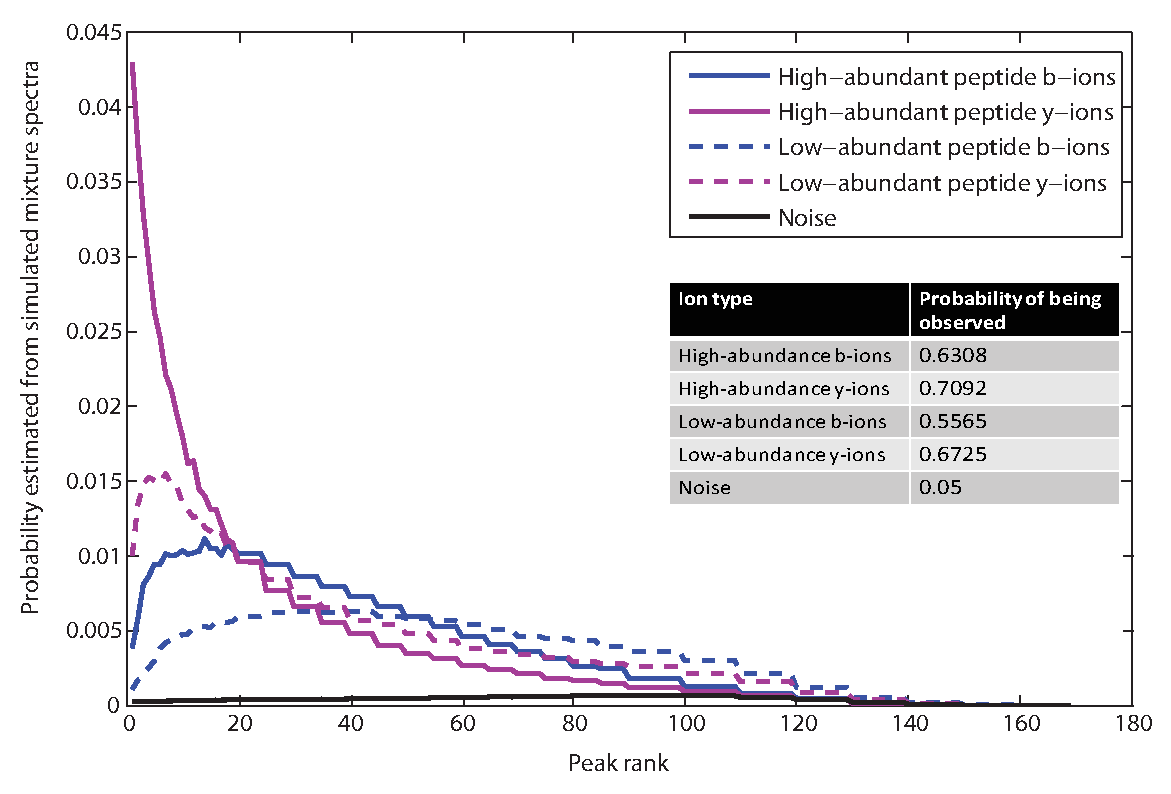
\includegraphics[height=75mm, width=120mm]{./Figures/MixDB_mixture_model_distibutions_expanded}
%		\caption{Framentation statistics for multiplexed spectra: {\footnotesize Statistics are computed from a set of simulated multiplexed spectra.  As shown in figure, fragment ions from high-abundance and low-abundance peptides in multiplexed spectra have different distribution of peak ranks (peak ranked from most intese to least intense). Scoring function that design only for single-peptide spectra do not capture this characteristic of multiplexed spectra.  Thus scoring function that distinguish and explicitly model fragment ions from high/low-abundance peptides in multiplexed spectra are used in MixDB.  Probability shown in the table is the total probability that a particular ion type is being observed in the training data, they correspond to the area under each curve.}}
%	\label{mix_peak_ranksdistr}
%\end{figure}
%
%%\subsubsection*{Classification of database search matches}
%To assess whether the top match is significant we use a two-stage classifier to distinguish true matches from false positive matches.  We consider three possible outcomes when searching a given query spectrum
%$S$: 1) No-match: $S$ does not match any peptide in the database; 2) Single-peptide match: $S$ matches one and peptide in the database; 3) Mixture-match: $S$ matches a pair of peptides in the database.  As described in MixDB~\cite{wang2011peptide}, classification of the top matches is done using two Support Vector Machine (SVM)~\cite{cortes1995support}. The first SVM distinguishes No-match cases from Single-peptide / Mixture matches and the second SVM distinguishes Single-peptide matches from Mixture matches.
%
%%\subsubsection*{Estimation of False Discovery Rates}
%False Discovery Rates (FDRs) were estimated by extending the standard Target-Decoy strategy for database search~\cite{Elias2007}. Depending on whether each peptide in the top peptide pair comes from the Target or Decoy databases, matches are divided into the following possibilities: \emph{TT} -- both peptides matched Target, \emph{TD} -- the most abundant peptide matched Target and the least abundant peptide matched Decoy, \emph{DT} -- the most abundant peptide matched Decoy and the least abundant peptide matched Target and \emph{DD} -- both peptides matched Decoy.  When searching multiplexed spectra there are two possible outcomes for identification: single-peptide matches and mixture matches, each with a separate corresponding FDR. The FDR for single-peptide matches is defined as: $FDR_{match} = \frac{{DT} + DD}{TT + TD}$ and the FDR for multiplexed-spectrum identification is defined as: $FDR_{mixture} = \frac{TD}{TT}$.  Note that DT and DD peptide pairs will never advance to the second SVM because they are rejected as false positives after $FDR_{match}$; only TD and TT matches are considered by the second SVM as candidate mixture matches.
%
%%The efficiency of the projected-spectrum filter is determined by the highest (i.e., worst) rank of a correct peptide match of a multiplexed spectrum to the database $D$.   Note that a correct match in $D$ is a match to one of the peptides generating $M$ -- single-peptide spectra have one correct match, multiplexed spectra have two correct matches and thus two correct-match ranks.
%%As shown in Figure \ref{Psimranks}, the resulting ranks of correct matches indicate that the projected-spectrum filter is an efficient filter that, for over $96\%$ of cases, retains \emph{both} correct matches (i.e., maximum ranks) at ranks less than 500 from about 10,000 candidate peptides (yeast database, 3~Da precursor mass filtering).  The left panel in Figure~\ref{Psimranks_mixdb} also shows that one of the correct matches, presumably the higher-abundance peptide in the multiplexed, almost always has rank less than 10 (i.e., minimum ranks).  This means that for almost all cases one only needs to pair the top 10 candidates with the top 500 candidates to find the correct match.  Using this strategy at most $10 \times 500 = 5000$ candidate pairs need to be considered, thus conferring a $\approx\frac{10,000 \times 10,000}{2 \times 5000} = 10,000\times$ speedup compared to considering all $\approx 5\times 10^7=\frac{10,000 \times 10,000}{2}$ possible candidate peptide pairs.
%As in M-SPLIT we evaluated the efficiency of the projected-spectrum filter by counting the number of peptide pair MixDB had to consider to find the correct matches and as shown in Figure~\ref{Psimranks2} the filtration achieve approximately a $10,000$ fold speedup.
%
%\begin{figure}[h!]
%	\centering
%		\begin{minipage}[c][60mm][c]{156mm}
%			\begin{tabular}[c]{cc}
%			\\[-2pt]
%			\begin{minipage}[c][60mm][c]{72mm}
%				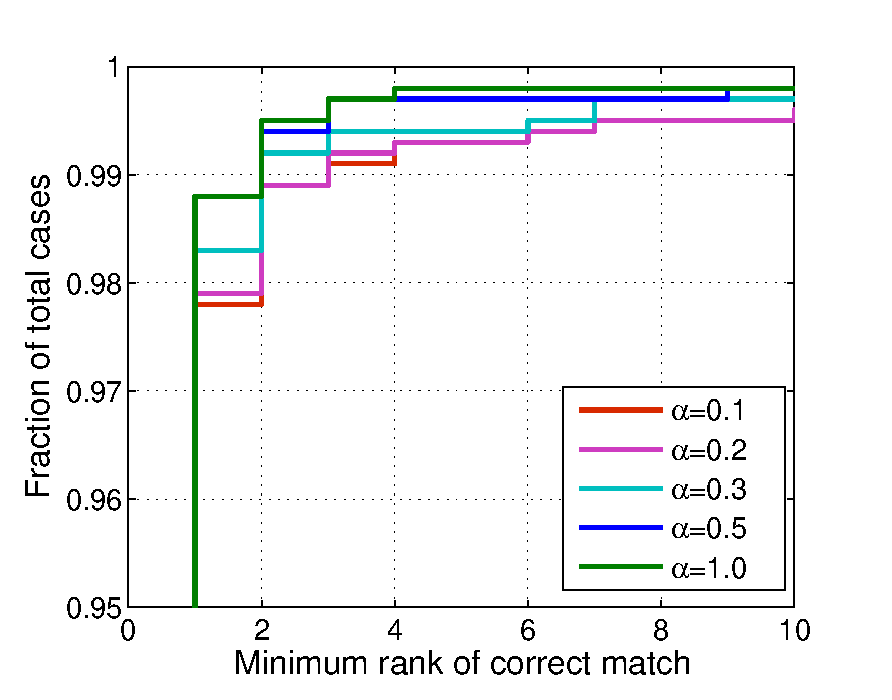
\includegraphics[height=60mm, width=72mm]{./Figures/MixDB_mixtureranks_min}
%			\end{minipage}
%			&
%			\begin{minipage}[c][60mm][c]{72mm}
%				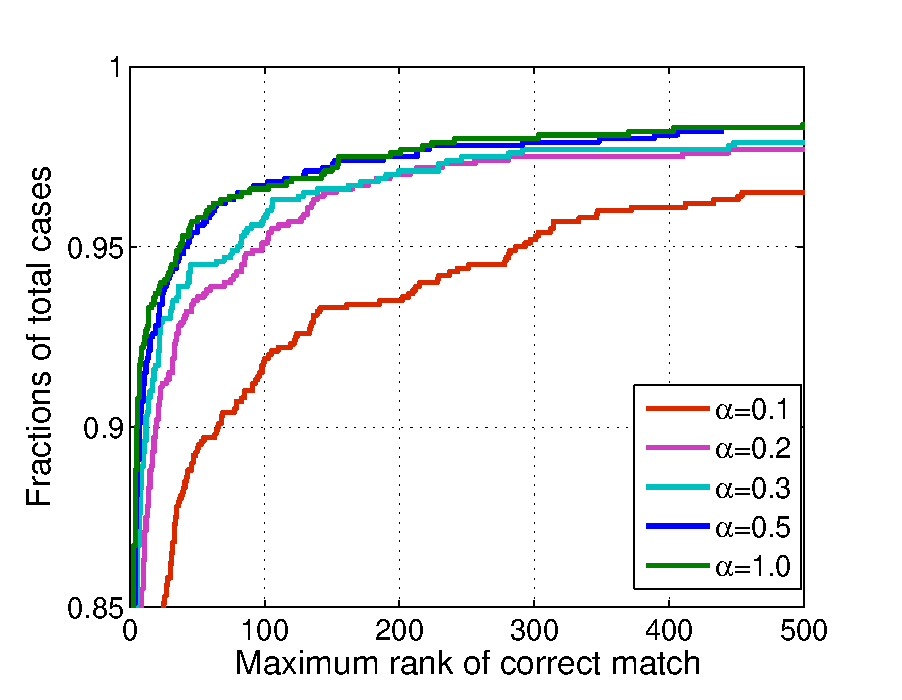
\includegraphics[height=60mm, width=72mm]{./Figures/MixDB_mixtureranks_max}
%			\end{minipage}
%		\end{tabular}		
%		\end{minipage}
%		\caption{Filtration efficiency:
%		 {\footnotesize Cumulative distributions of minimum rank (left) and maximum rank (right) for correct matches of simulated mixture spectra to the yeast database. Candidate peptides in the database are first sorted according to decreasing score against the corresponding projected multiplexed spectra (typical number of peptide candidates after precursor mass filtering is $\approx$10,000). The ranks of the correct matches are then determined. Correct matches are peptides in the database that correspond to one of the peptides used to generate the simulated multiplexed spectrum. Since each multiplexed spectrum has two correct matches we report both the minimum (i.e., best) and maximum (i.e., worst) rank of the two matches in the left/right panels, respectively. As shown, in more than 96\% of cases, one of the correct matches has rank $\le 10$ (left) while the other correct match ranks $\le 500$ (right).  Thus it is sufficient to pair the top 10 candidates with the top 500 candidates to find the correct pair.  Using this strategy at most $10 \times 500$ peptide \emph{pairs} need to be considered, resulting in a speedup of four orders of magnitude compared with considering all $\approx 5\times10^7$ possible peptide pairs.}
%}
%\label{Psimranks2}
%\end{figure}

%\subsubsection*{Benchmarking in simulated multiplexed spectra}
%We first evaluated the performance of the PPSM scoring model in a set of simulated multiplexed spectra and compared MixDB's %performance with an iterative search strategy where one first identifies the highest-scoring peptide, removes all annotated %peaks from the spectrum and then uses the ''residual'' spectrum to search against the database a second time to identify the %second peptide. This revealed~\cite{wang2011peptide} that when $\alpha$ is high, the performance of the iterative method is %comparable with that of the combined scoring function but, as $\alpha$ becomes smaller, the performance of the iterative %method becomes over $3-5\times$ worse than the proposed PPSM scoring model.
%
%We evaluated the performance of our scoring model in a set of simulated multiplexed spectra. The percentage of cases where the top peptide pair returned by MixDB is correct is shown in Table~\ref{tab:MixDB_toppair_correct}.   As expected, as $\alpha$ decreases the performance worsens because it becomes harder to identify the lower abundance peptide.
%We also compared the performance of MixDB with M-SPLIT and on average, M-SPLIT correctly identifies $15\%$ more multiplexed spectra than MixDB.  We also compare MixDB with an iterative search strategy where one first identifies the highest-scoring peptide, removes all annotated peaks from the spectrum and then uses the ''residual'' spectrum to search against the database a second time to identify the second peptide.  As we can see in Table ~\ref{tab:MixDB_toppair_correct} when $\alpha$ is high, the performance of the iterative method is comparable with that of the combined scoring function. However, as $\alpha$ becomes smaller, it is better to consider both peptides at the same time.
%
%\begin{table}[h!]
%  \small
%	\centering
%		\begin{tabular}[c]{ccccc} % centered columns (4 columns)
%			\hline % inserts single horizontal line
%			Mixture coefficient\\ ($\alpha$) & M-SPLIT & MixDB  & MixDB* & Iterative method\\
%			\hline
%			1:1 & 97 & 87 (97)  & 95 (98) & 81\\
%			1:0.5 & 92 & 79 (92) & 90 (98) & 74\\
%			1:0.3 & 80 & 66 (86) & 79 (92) & 57\\
%			1:0.2 & 63 & 50 (77) & 69 (87) & 30\\
%			1:0.1 & 34 & 19 (43) & 34 (70) & 6\\
%			\hline %inserts single line
%		\end{tabular}
%	\caption{{\footnotesize MixDB and M-SPLIT were evaluated on a set of 5000 simulated multiplexed spectra. Each row indicates the percentage of cases when the top ranking pair is correct; numbers in parenthesis indicate fraction of cases when one of the top ten peptide pairs is correct. Two types of database search were performed. In MixDB, each spectrum was searched against all Yeast tryptic peptides. In MixDB*, each spectrum was searched only against peptides with spectra in the NIST Yeast spectral library. }
%}
%	\label{tab:MixDB_toppair_correct}
%\end{table}
%
%\subsubsection*{Peptide identification in Yeast lysate data}

We  compared MixDB it with InsPecT~\cite{tanner05}, ProbIDtree~\cite{zhang2005tree} and M-SPLIT~\cite{wang2010msplit} on a Yeast lysate dataset~\cite{li2009}. For identification of single-peptide spectra, all three database search methods achieved comparable accuracy of $97\%$ while MixDB identified approximately 6\% more spectra than InsPecT and 21\% more spectra than ProbIDtree. This shows that MixDB's performance in identifying single-peptide spectra was not diminished by considering more than one peptide per spectrum.  For multiplexed spectra, MixDB identified $20\%$ more spectra than ProbIDtree while achieving a similar accuracy ($\approx 96\%$) as in single-peptide spectra. On the other hand, ProbIDtree accuracy drop to $\approx 90\%$ for multiplexed spectra.

%To illustrate the utility of our method, we tested our database search method on an experimental {\em Yeast dataset}~\cite{li2009}.  The data were analyzed using InsPecT~\cite{tanner05}, MixDB~\cite{wang2011peptide} and ProbIDtree~\cite{zhang2005tree} and M-SPLIT~\cite{wang2010msplit} with 3~Da parent mass tolerance.  The accurate precursor information was then used to estimate accuracy.
%%as well as utilizing the accurate precursor masses for a posteriori validation of search results.In short, InsPecT is able to identify a total of 22,658 single-peptide spectra, MixDB is able to identify 23,930 single-peptide spectra plus 978 multiplexed spectra and ProbIDtree is able to identify 19,840 single-peptide spectra plus 821 multiplexed spectra.  Again, The accurate precurosr mass was used to estimate the accuracy of the identification tools.  We first focus our attention on single-peptide cases.
%As shown in Table~\ref{tab:MixDB_yeast_compare}, for identification of single-peptide spectra, all three database search methods have comparable accuracy of $97\%$ while MixDB identifies approximately 6\% more spectra than InsPecT and 21\% more spectra than ProbIDtree. This shows that MixDB's performance in identifying single-peptide spectra was not diminished by trying to identify more than one peptide per spectrum.  For multiplexed spectra, MixDB identify $20\%$ more spectra than ProbIDtree while achieving a similar accuracy ($\approx 96\%$) as in single-peptide spectra. On the other hand, ProbIDtree accuracy drop to $\approx 90\%$ for multiplexed spectra.

%Two main reasons contribute to MixDB's higher precision.  First, MixDB only searches up to two peptides per spectrum (ProbIDtree attempts to look for up to eight peptides per spectrum), thus theoretically it has a smaller search space than ProbIDtree.  More importantly, MixDB applies different scores and FDRs for the first and second identified peptides in each MS/MS spectrum ($FDR_{match}$ and $FDR_{mixture}$, respectively).  This is crucial because high-abundance peptides are likely to have very different match statistics (e.g., \% explained intensity, \% b/y ions presented) than low-abundance peptides in multiplexed spectra. Because there are many more single-peptide spectra than multiplexed spectra in this dataset, applying a single global FDR for the combined identification of both single-peptide and multiplexed spectra can lead to an underestimation of FDR for multiplexed spectra.  Just as in the case of ProbIDtree, it has an estimated precision of $\frac{90.1\%\times821 + 97.8\%\times19840}{19840+821}=97.94\%$ or an overall FDR of $2.06\%$.  However, the precision for multiplexed spectra is only $90.1\%$, bringing its FDR on multiplexed spectra to 9.9\% which is much higher than its FDR for single-peptide matches. In summary, we show that MixDB has both higher sensitivity and precision than ProbIDtree in identifying multiplexed spectra while having comparable performance to InsPecT in identifying single-peptide spectra.

%\begin{table}[h!]
%	\small
%	\begin{tabular}{ccccccccc} % centered columns (4 columns)
%	      %\multicolumn{9}{l}{\small{Spectrum and peptide identifications in the Yeast dataset}}\\
%			  \hline
%              & \multicolumn{3}{c}{Spectrum Identifications} & \multicolumn{3}{c}{Unique Peptides} & \multicolumn{2}{c}{Accuracy}\\
%			  & Single-peptide & Multiplexed & Total & Single & Multiplexed & Total & Single & Multiplexed\\
%  			\hline % inserts single horizontal line
%  			MixDB &  23930 & 978 & 24908  & 5476 & 1128 & 5802  & 98.3\% & 95.9\%\\
%  			ProbIDtree & 19840 & 821 & 20660 &  4420 & 820 &  4739 & 97.8\% & 90.1\%\\
%  			InsPecT  & 22658 & n/a &  22658 & 5272 &  n/a & 5272 & 97.1\% & n/a\\
%			  M-SPLIT  & 	28417 & 2567 & 30984  & 5997 & 2394 & 6684 & 97.3\% & 95.4\%\\
%			 \hline
%		\end{tabular}\\
		
%	\begin{tabular}{ccccccc} % centered columns (4 columns)
%	      \multicolumn{7}{l}{a) \small{Spectrum and peptide identifications in the Yeast dataset}}\\
%			\hline
%              & \multicolumn{3}{c}{Spectrum Identifications} & \multicolumn{3}{c}{Unique Peptides}\\
%			  & Single-peptide & Multiplexed & Total & Single-peptide & Multiplexed & Total\\
%  			\hline % inserts single horizontal line
%  			MixDB &  23930 & 978 & 24908  & 5476 & 1128 & 5802\\
%  			ProbIDtree & 19840 & 821 & 20660 &  4420 & 820 &  4739  \\
%  			InsPecT  & 22658 & n/a &  22658 & 5272 &  n/a & 5272\\
%			  M-SPLIT  & 	28417 & 2567 & 30984  & 5997 & 2394 & 6684\\
			 % SpectraST &  33102 & n/a  & 33102 &  6493  & n/a & 6493 \\
			 % SpectraST* & 25723 & n/a  & 25723	& 5827 & n/a & 5827
%			 \hline
%		\end{tabular}\\
%		%*SpectraST results after adjusting F-score threhold to bring SpectraST precision to 97\% \\as estimated for the other methods.\\
%%		\\\\
%%				\begin{tabular}[c]{ccc} % centered columns (4 columns)            \multicolumn{3}{l}{b) \small{Estimated precision in the Yeast dataset}}\\
%%			\hline % inserts single horizontal line
%%			Method & Single-peptide matches &  Multiplexed matches \\
%%			\hline % inserts single horizontal line
%%			MixDB &  98.3\% &  95.9\% \\
%%			ProbIDtree & 97.8\% &   90.1\%  \\
%%  		InsPecT   &  97.1\% &  n/a \\
%%			M-SPLIT   &  97.3\% &  95.4\% \\
%			%SpectraST &  95.0\% &  n/a      \\
%%			\hline
%%		\end{tabular}
%	\caption{ {\footnotesize Search results on the Yeast dataset for MixDB, M-SPLIT, InsPecT and ProbIDtree.  Numbers of identified spectra (single-peptide and multiplexed) and unique peptides are compared. To allow for identification of co-eluting peptides, all searches were run using 3 Da precursor mass tolerance.  The accurate precursor mass information was then used a posteriori to estimate the precision of peptide identification by comparing the theoretical precursor m/z of peptides returned by each method and the observed precursor m/z values in the corresponding MS1 scan (isotopic profile). An identification is considered correct if the difference between theoretical and experimental precursor m/z values is less than 5~ppm.}}
%	\label{tab:MixDB_yeast_compare}
%\end{table}


\subsubsection{Extending scoring models to more than two peptides}

The development of probabilistic scoring models in MixDB~\cite{wang2011peptide} demonstrated that scoring models for mPSMs should have several desirable properties. First, in contrast with the case of single-peptide spectra, this scoring model should consider that fragment ions from other peptides are possible in the same spectrum and thus it should not penalize unmatched peaks simply as noise.  Second, the scoring model should also be aware of the relative abundance of the peptides present in the multiplexed spectrum.  As shown with MixDB, high-abundance peptides and low abundance peptides have significantly different peptide fragmentation statistics. Finally, the scoring model should also account for the dependencies among different peptide candidates matched to the same multiplexed spectrum, rather than treating each peptide candidate as an independent match.  A scoring function without this feature will likely give artificially high scores to sets of peptide candidates with significant overlap of theoretical fragment ion masses.
% since spectrum peaks of the same or similar mass will be awarded match scores multiple times.

MixDB uses different scoring models for the more and less abundant peptides in a spectrum.
Since multiplexed spectra  may originate from a varying number of peptides, it is not practical to develop separate scoring models for each of $n$ spectra in an $n$-tuple mPSM.  Instead, we expect that peptides with similar relative abundances in a multiplexed spectrum will likely have similar fragmentation statistics.  Thus we propose to derive scoring models $\text{Score}(M,P,A_{P})$, for matching a peptide $P$ with relative abundance $A_{P}$ against a multiplexed spectrum $M$. $\text{Score}(M,P,A_{P})$ will have a different set of scoring parameters for each range of peptide abundance.  Different strategies can be used to model peptide abundance. For example, the total ion intensity putatively assigned to peaks from a particular peptide in the multiplexed spectrum can be divides into different categories if it falls in a particular bin with boundaries defined at 5000, 7500, 10,000, 20,000 and 50,000 ion counts. The actual thresholds will depend on the type of instrument and fragmentation method used to generate the MS/MS spectra and will be learned from empirical data.
This will be done from annotated multiplexed MS/MS spectra (e.g., the SWATH dataset described above).
% or, in the worst case scenario, by using simulated multiplexed spectra by linearly combining single-peptide spectra as %before~\cite{wang2010msplit,wang2011peptide}.

In order to reduce the influence of peaks from other peptides in a multiplexed spectrum, we have shown that projected-spectrum cosine is a good way to focus on one particular peptide for spectral library searches.  Thus, rather than scoring a peptide candidate directly against a multiplexed spectrum, we instead propose to extend database search to first score peptide candidates against their corresponding projected-spectrum.  Specifically, let $S(P)$ be the theoretical spectrum for peptide P with non-zero intensities only at theoretical ion masses and let $M^P$ be the projected-spectrum of $M$ on $S(P)$ as defined above for spectral library searches. We note that since peaks are removed from $M$ to obtain $M^P$, the ranks of the peaks in $M^P$ keep their relative order but their numeric range is reset to start from 1 until the number of non-zero bins in $M^P$. We then have:

\begin{eqnarray*}
\text{Score}(M,P,A_{P})=\text{Score}(M^P,S(P),A_P) = \sum_{i=1}^{n}{\text{Score}(m^p_i,s(p)_i,A_P)}
\end{eqnarray*}

To score a tuple of peptide candidates $C=(P_1, ..., P_k)$ against $M$, we first compute the scores for each candidate peptide $P_i$ matched to its corresponding projected spectrum $M^{P_i}$ and then combine these scores element-wise to obtain a final mPSM score:

\begin{equation*}
\text{Score}(M,(P_1,..., P_k),(A_{P_1},..., A_{P_{k}})) = \sum_{i=1}^{n}{\max(\text{Score}(m^{p_{1}}_i, s(p_1)_i,A_{P_{1}}),..., \text{Score}(m^{p_k}_i, s(p_k)_i, A_{P_k}))}
\end{equation*}

The element-wise operation used to combine the scores can be any operation handling the dependencies among different candidate peptides matched to the multiplexed spectrum so that scores will not be double-counted. We use $\max$ as an example from MixDB but it is not the only solution. For example, other possibilities include $i)$ evenly splitting the scores for a particular peak among all the theoretical fragments matched to that peak or $ii)$ weighting the scores by the relative abundance of the peptides.

\subsubsection{Greedy algorithm for identification of multiplexed spectra}

In addition to developing scoring functions for multiplexed spectra, we will also need optimized search strategies to navigate the vast search space of all possible combinations of peptides to be matched against each multiplexed spectrum.  Notice that the main idea behind the search strategy in MixDB is also a greedy search algorithm: it first finds the top-scoring single-peptide candidates, then pairs each of these candidates with the remaining candidates in the database to find the best matching pair. This procedure can be generalized as follows -- once we find the best $k$-tuple of peptide candidates, it can be extended with the next-best peptide candidate to define a $k+1$-tuple of peptide candidates. This operation can be repeated any number of times. As shown with MixDB~\cite{wang2011peptide}, in practice the best pair of candidates does not always contain the best-scoring single-peptide candidate. Thus we relax the condition slightly and during the $j^{th}$ round of searching we will retain the top $N_{j}$ candidates. The actual parameters $N_{j}$ will be determined empirically from experimental data.  We note that this search strategy is different from the iterative strategies proposed in the past where one first identifies the best-scoring single peptide, removes the peaks corresponding to that peptide and then uses the ``residual'' spectrum for another round of search. As shown in \cite{wang2011peptide}, such subtractive strategy has lower sensitivity because it sometimes removes peaks that are best assigned to a different peptide and thus leads to lower identification rates for subsequent round of searchings.  By considering all peptide candidates at the same time, our approach leaves it to the mPSM probabilistic scoring model to infer which fragment ions most likely generate each observed peak.

Each round of search using this strategy can add one more candidate peptide to the $k$-tuple matched to the multiplexed spectrum.  In M-SPLIT, whether the second peptide is a significant match to the multiplexed spectrum is determined by the significance of the second peptide's resulting increase in the multiplexed match cosine score.  Similarly, the proposed search procedure can be stopped when the additional peptide does not increase the total score by more than a certain threshold.  Alternatively we can also halt the search when the explained intensity in the multiplexed spectrum exceeds a predetermined threshold.
%Independently of these, one can also estimate an upper bound for the number of peptides present in a multiplexed spectrum %ahead of the search by analyzing the isotopic profile of precursors in the survey scan for that particular multiplexed MS/MS %spectrum.

%\begin{itemize}
%    \item Use rank models per peptide abundance (i.e. alpha) quartiles: bottom, mid-low, mid-high, high
%    \item Projected ranks extensions for K peptides
%    \item Filtering??
%\end{itemize}

\subsection{Aim 3: Computing statistical significance for mPSMs}

CCMS developments in the previous cycle demonstrated that MixDB
%can accurately and efficiently
 identifies  significantly more multiplexed spectra~\cite{wang2011peptide} than other tools.  However it still only identifies about half as many multiplexed spectra as our multiplexed spectral library search tool M-SPLIT~\cite{wang2010msplit}. Comparison of the results between the two methods reveals that current version of MixDB suffers from relative low sensitivity due to its limited ability to separate true matches from false positives \-- a difficult question even in the case of single-peptide spectra~\cite{kall2007semi,kim2008spectral,nesvizhskii2010,gupta11}.  Capitalizing on recent advances using a generating function approach to rigorously compute the statistical significance of PSMs, we propose to extend the MS-GF~\cite{kim2008spectral} approach from PSMs to mPSMs. Below we first show how to rigorously compute statistical significance of a PPSM in multiplexed spectra and later generalize it to mPSM.

%\subsection*{PRM scoring model for multiplexed spectrum}

As before, we represent a spectrum as a real-valued vecto: $V = v_{1} ... v_{N}$, where $v_{i}$ is the sum of intensities of all the peaks with masses between $i-0.5$ and $i+0.5$. Similarly to TRD4, a prefix residue mass (PRM) spectrum represents a transformation of  spectrum into its scored version $S = s_{1} ... s_{N}$ using a probabilistic model~\cite{kim2009}(see TRD4).
%At every mass position $i$ of the PRM spectrum is a score $s_{i}$ that represents the log-likelihood that the peptide from %which the spectrum was generated contains a prefix mass $i$~\cite{dancik99}. Given a peptide P, its prefix masses are defined %by the sum of amino acid masses for each peptide prefix.
For a peptide $P$ with prefix masses $p_{1} .... p_{n}$,  the score of matching peptide $P$ to a spectrum $S$ is the sum of all the scores at its theoretical prefix masses in the PRM spectrum: $\text{Score}(P,S) = s_{p_{1}} + s_{p_{2}} ... + s_{p_{n}}$.

\subsubsection{Spectral probability for PPSM}

We first consider a multiplexed spectrum as a spectrum from two peptides. When interpreting a multiplexed spectrum $M$, we construct two PRM spectra, $M^{H}$ and $M^{L}$, to represent the two scoring models for the high and low-abundance peptides present in the multiplexed spectrum, respectively.  As we showed in MixDB, different scoring models are needed for high and low-abundance peptides because they were shown~\cite{wang2011peptide} to have distinct fragmentation statistics.  When matching a multiplexed spectrum ($M$) against a pair of peptides ($P$, $Q$) we assume the first peptide is the high-abundance peptide.  Thus the score of a pair of peptides ($P$, $Q$) against a multiplexed spectrum $M$ will be the sum of scoring $P$ with $M^{H}$ and scoring $Q$ with $M^{L}$: \text{Score}($P$, $Q$, $M$) = $M^{H}_{p_{1}} + ... M^{H}_{p_{n}} + M^{L}_{q_{1}} + ... M^{L}_{q_{n}}$. To avoid double counting, when a prefix mass of $P$ is the same as a prefix mass of $Q$, only the bin with the higher score is considered and the other peptide gets a score of zero for that particular mass position.

The statistical significance of a particular peptide $P$ matched to a spectrum $S$ with score $T$ is determined by the probability that a random peptide (out of all possible peptides), when matched to $S$, has a score greater or equal than $T$. We will refer to this as the \emph{Single-peptide probability} in order to better distinguish it from the other definitions introduced below.   Analogously, to compute the statistical significance of a particular peptide pair ($P$,$Q$) matched to a multiplexed spectrum ($M$) with a score of $T$, we are interested in two statistical questions:

\begin{itemize}
\item \emph{Joint-probability}: What is the probability that a random peptide pair (out of all possible peptide pairs), when matched to $M$, yields a score greater than  $T$?

\item \emph{Conditional-probability}: Given a peptide $P$, what is the probability that a random peptide $Q$ (out of all possible peptides) together with $P$, when matched to $M$, yields a score greater than  $T$?
\end{itemize}

Intuitively we are interested in finding cases where both peptides $P$ and $Q$ are statistically significant matches to a spectrum $M$. We address this question in two steps.  \emph{Joint-probability} assesses the probability  that two random peptides can have the same or higher score than the current best match.  When this probability is very low, this means that at least one peptide is a significant match to the spectrum. Once we assume that at least one peptide is a true match, \emph{Conditional-probability} helps us to evaluate whether the second peptide is also a statistically significant match.

In order to compute the score distribution for all peptides, MS-GF~\cite{kim2008spectral} uses a dynamic programming approach to compute the Single-peptide probability efficiently without explicitly computing the scores for all peptides.  Here we extend this generating function approach to compute the probability for \emph{Joint} and \emph{Conditional} probabilities.
Let $J_M(p_{i}, q_{j}, T)$ be the Joint-probability that a pair of peptides $P$, $Q$ with parent mass $p_{i}$ and $q_{j}$ match to $M$ with score higher than or equal to $T$. When there are no shared peaks between $P$ and $Q$ this means $P$ matches to $M^{H}$ up to the $p_{i}^{th}$ bin and $Q$ matches to $M^{L}$ up to $q_{j}^{th}$ bin.  %Also recall that $M^{H}$ and $M^{L}$ represent the PRM spectra for the high and low abundance peptides, respectively.
We  define the following recurrence relationship for Joint-probability:

\begin{equation}
J_M(p_{i},q_{j},T) = \left\{
\begin{array}{l}
  if\ p_{i} < q_{j}: \\
      \displaystyle\sum\limits_{all\ amino\ acids\ a}{J_M(p_{i}, q_{j} - |a|, T - M^{L}(q_{j}))\times \Pr(a)} \\
  if\ p_{i} > q_{j}:\\
      \displaystyle\sum\limits_{all\ amino\ acids\ a}{ J_M(p_{i} - |a|, q_{j}, T - M^{H}(p_{i}))\times \Pr(a)} \\
  if\ p_{i} == q_{j}: \\
  \sum\limits_{a_1}{\sum\limits_{a_2}{J_M(p_{i} - |a_1|, q_{j} - |a_2|,
        T - \max \left\{
                  \begin{array}{c}
                   M^{H}(p_{i}) \\
                   M^{L}(q_{j})
                  \end{array}
                 \right\})}} \\
                 \ \ \ \ \ \ \ \ \ \ \times \Pr(a_1) \times \Pr(a_2)
\end{array}
\right\}
\label{mixgf.dprec}
\end{equation}

In the equation above, $a$, $a_1$, and $a_2$ denote amino acids; $|a|$ denotes the mass of an amino acid and $\Pr(a)$ denotes the probability that a particular amino acid occurs in a peptide.  When considering all possible peptide sequences this probability is uniform and has a value of $\frac{1}{20}$ for each of the 20 standard amino acids. To better reflect the amino acid composition observed in real protein sequences we can also obtain this probability by computing the frequency of each amino acid in the protein sequence database against which the spectra are searched.  To start the computation of the recurrence, we initialize $J_M(0,0,0)=1$.

The computation of the Conditional-probability is very similar to that of Single-peptide probability, except that it is conditioned on the first peptide being accepted as a match. % thus when a prefix mass of the second peptide is equal to a prefix mass of the first peptide, one only uses the score of the mass position with higher score.
Specifically, for a peptide pair ($P$, $Q$),  matched to a spectrum $M$ with score $T$, we define that peptide $P$ and $Q$ contribute $T_{P}$ and $T_{Q}$ to the total score, respectively. Assuming that peptide $P$ was matched to $M$, we define $C_M(q_{j}, T | P)$ as the Conditional-probability that a peptide with parent mass $q_{j}$ together with $P$ match $M$ with a score greater than or equal to $T$. To compute this probability, we first modify $M^{L}$ by setting all the bins corresponding to a prefix mass of $P$ to zero if $M^{H}$ has a higher score at the same location.
%$when: p_{i} == q_{j}\ \ \ \ M^{L}(q_{j}) = 0\ \ if\ M^{L}(q_{j}) < M^{H}(p_{i})$ \\
Then the Conditional-probability is given by the following recurrence:

\begin{equation*}
C_M(q_{j},T | P) = \sum\limits_{\text{all\ amino\ acids\ a}}{C_M(q_{j} - |a|, T - M^{L}(q_{j}) | P)}\times \Pr(a)
\end{equation*}

We initialize the recurrence with the base case: $C_M(0, T_{P} | P) = 1$.  The base case starts at score $T_{P}$ rather than zero because the first peptide $P$ already contributes $T_{P}$ to the total score.

We note that even though the Joint-probability assesses whether at least one peptide is a significant match to the spectrum, it does not determine which peptide is the significant match in the case only one peptide is significant match.  More importantly, when calculating the Conditional-probability one assumes that the first peptide is a true match but it is unclear which peptide is the first peptide from the Joint-probability assessment. In order to resolve this ambiguity, for a candidate peptide pair ($P$,$Q$) matched to a spectrum $M$, we compute their respective Single-peptide probabilities and the peptide with lower (i.e. statistically more significant) Single-peptide probability is designated as the first peptide.

{\bf Approximating joint probability of PSM.} The dynamic programming approach above enables us to compute the \emph{Joint-probability} without explicitly computing the scores for all peptide pairs. However the computational complexity still scales exponentially with the number of peptides that generated the observed spectrum (e.g., quadratic for two peptides).  Thus it is desirable to find a way to approximate this probability efficiently. To derive this approximation we borrow an intuition from the definition of conditional probability where the joint probability of two random events $(P,Q)$:
%, is equal to the probability of one event times the conditional probability of the second event given the first event:
 $\Pr(P\ \wedge\ Q) = \Pr(P)\times \Pr(Q|P)$. Analogously we can decompose the Joint-probability question into two simpler questions: 1) what is the probability of finding a random peptide that matches to $M$ with a score larger than $T_{P}$? and 2) once we find a first peptide $P$ what is the probability of finding a random peptide that together with $P$ scores  higher than $T$ when matched to $M$?  Note that the first question is just the \emph{Single-peptide probability} and the second question can be answered with the \emph{Conditional-probability}. Therefore we can define the following approximation:
$J_M(P,Q,T) \approx Single_M(P,T_{P}) \times C_M(Q,T| P)$. We refer to this approximation as the \emph{Product-probability}. While this formulation is not exactly equivalent to the definition of Joint-probability (because it does not explicitly consider the dependencies between all possible {\em pairs} of peptides that can be matched to the multiplexed spectrum), both Single-probability and Conditional-probability can be computed efficiently in linear time and we show below that this approximation is sufficiently accurate for our main use of Joint-probability -- to separate correct matches from false positive matches to multiplexed spectra.

%\subsubsection*{Preliminary Results}

{\bf Separating true and false multiplexed spectrum matches.} For a multiplexed spectrum that comes from two peptides, the top-scoring PPSM returned by database search methods may fall into three categories: 1) \emph{Correct-matches}: both peptides are correct matches; 2) \emph{Half-correct matches}: one peptide is correct and the other peptide is an incorrect match; 3) \emph{Incorrect-matches}: both peptides are incorrect matches.
Our goal is to separate correct matches from the other two types of matches.  To test the performance of our approach in this task, we constructed a set of simulated multiplexed spectra by linearly combining pairs of single-peptide spectra.  %Since we know a priori the peptides that generated each simulated multiplexed spectrum, we can extract the top-scoring correct, half-correct and incorrect matches returned by MixDB and compute their Joint and Conditional-probabilities.
As shown in Figure~\ref{separate}a, Joint-probability separates well between correct and incorrect matches.  However, there is considerable overlap between the Joint-probability of correct-matches and half-correct matches (Figure~\ref{separate}b).  Further investigation of cases in the overlap region shows that for correct-matches usually both peptides contribute moderate scores to the final combined score.  On the other hand,  for the half-correct matches, the correct peptide often contributes a very high score and thus even when paired with an incorrect match, the resulting combined high score still yields a low Joint-probability. Intuitively in order to separate half-correct matches from correct matches we need to look for cases that have high combined score as well as both peptides contributing significantly to the total score.  The concept of Conditional-probability defined above aims to address  this question - is the score of the peptide pair $(P,Q)$ significantly higher than that of the single peptide $P$? As illustrated in Figure~\ref{separate}c, Conditional-probability indeed is a better feature to separate correct matches from half-correct matches. Therefore a two-step procedure can be used to separate correct matches from false matches: at the first stage Joint-probability is used to filter out incorrect matches and then Conditional-probability is used to filter out half-correct matches.

\begin{figure}
	\centering
	 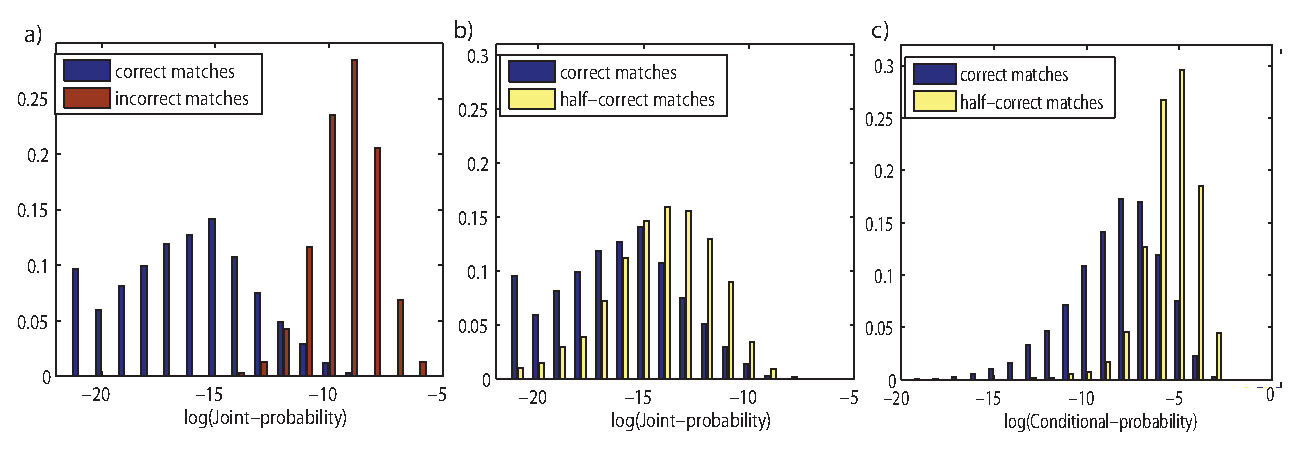
\includegraphics[height=45mm, width=135mm]{figures/MixGF_separation_true_false_matches}
		\caption{\footnotesize {\bf Separating true matches from false matches.}
		Multiplexed spectra were simulated by a linear combination of two single-peptide spectra. Correct matches are cases where both peptides in a PPSM are correct; incorrect matches are cases where both peptides are incorrect and half-correct matches are cases where one peptide is correct and one peptide is incorrect. The distribution of Joint-probability and Conditional-probability for correct matches (blue bars) incorrect matches (red bars) and half-correct matches (yellow bars) are shown.  As shown in a), the distributions of Joint-probability are well-separated between correct and incorrect matches. However, there is considerable overlap between the Joint-probability distribution of correct matches and half-correct matches (see b).  On the other hand, Conditional-probability is a better approach for separating correct matches from half-correct matches as shown in c).}
\label{separate}
\end{figure}

{\bf Joint-probability improves the detection of multiplexed spectra.}
For multiplexed spectra, we expect Joint-probability to perform better at separating correct from incorrect matches by explicitly considering two peptides. %Intuitively we expect that Single-peptide probabilities for correct peptide matches to multiplexed spectra to be higher (i.e. worse) than those for correct matches to single-peptide spectra.  This is because the presence of a second peptide in mixture spectra which will allow more peptides to match to the spectrum with high score. However for false matches the Single-peptide probability distribution remains roughly the same for both single-peptide and mixture spectra because they are random matches in either case.  Therefore the distribution of Single-peptide probabilities between correct and incorrect matches should be less well-separated for mixture spectra than for single-peptide spectra.
%Further analysis shows that this can be explained by the fact that in the Yeast dataset, most mixture spectra have the second peptide at relatively low abundance (we estimated that on average, the low-abundance peptides are at $1/3$ of the intensity of the high-abundance peptides~\cite{wang2010msplit}).  When the second peptide in the mixture is at relatively low abundance, the mixture spectrum tends to be more similar to a single-peptide spectrum and thus the ability to separate \emph{correct} from \emph{incorrect matches} using either Joint or Single-peptide probability is similar in these cases.
To show this, we generated a series of simulated mixture spectra where the first peptide is mixed with a second peptide at 100\%, 50\%, and 30\% of the first peptide's total intensity and then computed the Single-peptide probability, Joint-probability and Product-probability for the correct matches as well as the top-scoring incorrect matches. The performance of each probability function in separating correct from incorrect matches is shown in Table~\ref{tab:mixgf_stage1}.  When the second peptide is at relatively low abundance (i.e. 30\%), the performance of Single-peptide and Joint-probability is similar. However as we increase the relative abundance of the second peptide, Joint-probability performs considerably better at separating correct matches from incorrect matches.  Thus we expect that as multiplexed spectra with more peptides become more common, Joint-probability and its approximation will substantially improve our ability to identify multiplexed spectra.

\begin{table}
    \small
	  \centering
		\begin{tabular}{p{1.5cm}|p{3.3cm} p{1.5cm} p{1.5cm} p{1.5cm}} % centered columns (4 columns)
			\hline
         & Probability  & \multicolumn{3}{l}{False discovery rate (FDR)} \\
			          &               & 1\%  & 2\% & 5\% \\%& 10\%  \\
  			\hline \noalign{\smallskip}
  			$\alpha=1.0$ & Single-probability  & 71.9 & 74.7 & 81.8 \\%& 86.8 \\
  			             & Joint-probability   & 93.4 & 94.7 & 96.6 \\%& 97.6 \\
  			             & Product-probability & 93.6 & 94.0 & 96.7 \\%& 98.1 \\
  		  \hline \noalign{\smallskip}
  			$\alpha=0.5$ & Single-probability  & 85.7 & 87.5 & 92.0 \\%& 93.9 \\
  			             & Joint-probability   & 93.5 & 94.3 & 96.0 \\%& 98.1 \\
  			             & Product-probability & 92.6 & 94.1 & 96.1 \\%& 97.9 \\
  			\hline \noalign{\smallskip}
  			$\alpha=0.3$ & Single-probability  & 89.4 & 90.8 & 92.8 \\%& 93.8 \\
  			             & Joint-probability   & 90.2 & 91.8 & 93.8 \\%& 95.3 \\
  			             & Product-probability & 90.4 & 91.7 & 93.8 \\%& 95.6 \\
  			\hline
		\end{tabular}
		\caption{  {\footnotesize A set of simulated paired-peptide multiplexed spectra were constructed with mixture coefficients $\alpha=1.0, 0.5$ and $0.3$.
		Single-probability, joint-probability and product-probability were computed for the correct matches as well as the top-scoring
		incorrect matches returned by MixDB. Then each probability was used to separate correct from incorrect
		matches.  The sensitivity of accepting correct matches at different FDR levels is shown.}}
	%The numbers of single-peptide as well as mixture spectra and total numbers of unique peptides identified are compared.
	\label{tab:mixgf_stage1}
\end{table}


{\bf Approximating Joint-probability using Product-probability.} % Since the Joint-probability is computationally expensive and we evaluate whether Product probability can approximate it accurately.
As shown in Figure~\ref{approximate}.
%in most cases the Joint-probability is accurately approximated by Product-probability as most data points clustered tightly along %the main diagonal.
 For correct matches, the Product-probability is sometimes lower than the true Joint-probability.
%This can be attributed to the fact that the approximation does not explicitly consider all pairs of peptides \-- since $P$ is fixed %there are less opportunities for false positive matches to achieve high scores and thus the resulting spectral probability can be %smaller in such cases.
%did not explicitly consider all the dependencies between the two peptides.
However, the range of probabilities where this underestimation occurs is well below the range where incorrect matches tends to occur.  Therefore for the purpose of separating correct matches from incorrect matches, using the approximation is nearly equivalent to computing the exact Joint-probability.
%As shown in Figure \ref{approximate}b, correct matches and incorrect matches remain very well-separated whether using the %Product or Joint-probability.

\begin{figure}[!htp]
	\centering
	 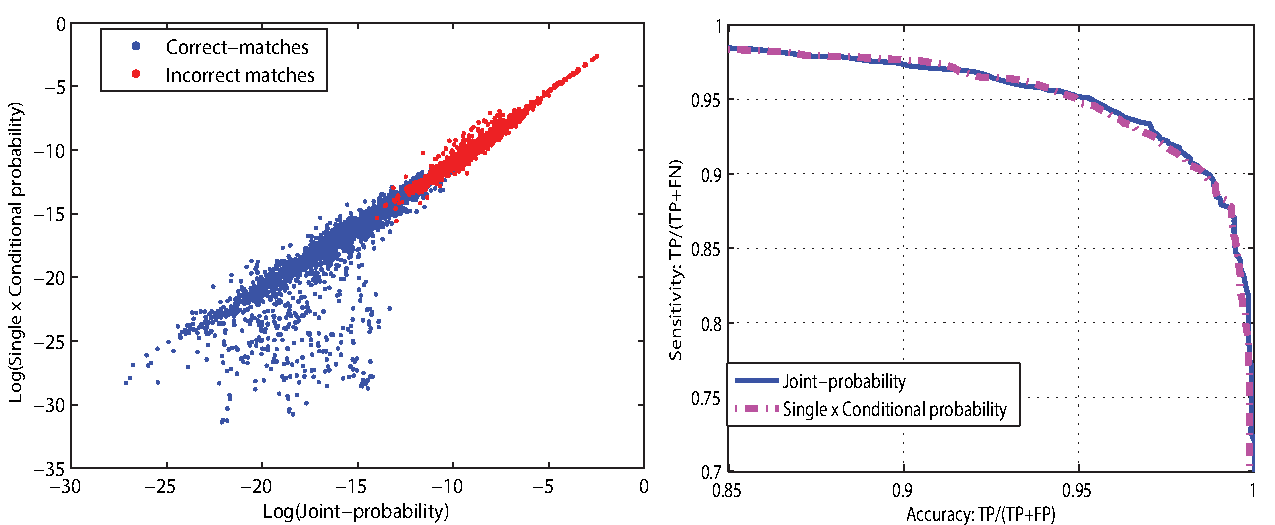
\includegraphics[height=45mm, width=125mm]{figures/MixGF_approx_joint_by_product_distrib_plus_ROC}
		\caption{\footnotesize {\bf Approximation of Joint-probability.}
  	Since it is computationally expensive to compute the exact Joint-probability for a multiplexed spectrum (scales exponentially with the number of peptides), we approximate it using Joint-probability defined as the product of Single-peptide and Conditional probabilities, which can be computed in linear time. As shown in a): for most cases the Product-probability accurately approximates the Joint-probability (most points cluster tightly around the main diagonal).  For correct-matches, there are some cases falling below the main diagonal. This shows that the approximated probability is sometimes lower than the true Joint-probability for correct matches.  However, for the practical purpose of distinguishing correct-matches and incorrect-matches, the two distributions remain very well separated using either the exact Joint-probability or its approximation as shown in the Precision/Recall curve on the right.}
\label{approximate}
\end{figure}

{\bf Preliminary results using a pilot implementation.} To assess the performance of our approach for identification of multiplexed spectra from two peptides, we tested it on a DDA Yeast cell lysate dataset~\cite{li2009} known to contain spectra from co-eluting peptides~\cite{wang2010msplit}.  We compared our pilot with two algorithms  for identification of multiplexed spectra (MixDB and ProbIDtree) and obtained encouraging results as shown in Table~\ref{tab:MixGF_ids_compare}.%, the proposed approach is able to outperform MixDB and ProbIDtree by identifying 26-76\% and 110-162\% more multiplexed spectra at the same FDR, respectively.
We also compared different options in which a different probability function was used at stage one to separate correct from incorrect matches.  These were all followed by using Conditional-probability at the second stage to separate correct matches from half-correct matches.  We observed that the performance when using the Joint-probability and its approximation (Product-probability) is very similar, further indicating that the approximation of the joint probability is accurate as a score for FDR-controlled identifications.
%One exception to that is at 1\% FDR, using Joint-probability at the first stage identifies more multiplexed spectra than Product-probability. We note that this might be due to an artifact of using TDA to estimate FDR since at 1\% FDR, there can be only a very small number (i.e. 5-13 spectra) of decoy multiplexed spectra allowed to pass the FDR threshold.  Thus, a small random fluctuation in the number of decoy spectra passing the FDR threshold results in a relative large change in FDR estimation.  As we allow for slightly higher FDR (such that small fluctuations in the numbers of decoy spectra passing the FDR threshold no longer significantly influence the FDR estimation) we see that using Joint-probability and Product-probability results in very similar performance.

\begin{table}
  \small
	\begin{center}
	  \begin{tabular}{p{6.5cm}|p{1.2cm}p{1.2cm}p{1.2cm}p{1.2cm}p{1.2cm}} % centered columns (4 columns)
			\hline
              & \multicolumn{5}{c}{False discovery rate (FDR)} \\
			 % & Single-peptide & Mixture & Total & Single-peptide & Mixture & Total\\
			      & 1\%  & 2\% & 3\% & 4\% & 5\%  \\
  			\hline
  			\noalign{\smallskip}
  			ProbIDtree & 504  & 773  & 923 & 1029  & 1272 \\
  			MixDB      & 748 & 1214 & 1620 & 1905 & 2124  \\
  			Pilot (Joint-probability)          & 1320 & 1580 & 1972 & 2268 & 2676 \\
  			Pilot (Product-probability)        & 1011 & 1646 & 2038 & 2356 & 2688 \\
			Pilot (Single-peptide probability) & 1310 & 1664 & 2091 & 2452 & 2760\\
			\hline
		\end{tabular}
  \end{center}
		%*SpectraST results after adjusting F-score threhold to bring SpectraST precision to 97\% \\as estimated for the other methods.\\
	\caption{{\footnotesize Numbers of paired-peptide spectra identified in a DDA Yeast dataset by ProbIDtree, MixDB and our pilot implementation of the proposed approach.  The different variants of the pilot differ by the type of probability (indicated in parenthesis) that is used in the first stage to separate correct matches from incorrect matches.  It is always followed by using Conditional-probability in the second stage to separate correct matches from half-correct matches.} }
	\label{tab:MixGF_ids_compare}
\end{table}

{\bf Extending the generating function to more than two peptides.} The proposed approach will be extended to compute the generating function for $k$ peptides matched to a spectrum $M$ by (1) applying the PRM scoring models proposed in aim 2 (instead of using the simplistic $M^H$/$M^L$ models specific to paired-peptide spectra) and (2) increasing the number of dimensions in the dynamic programming recursion from 3 to $k+1$ dimensions. As exemplified by the 3-dimensional recursion in Eq.~\ref{mixgf.dprec} for the 2-peptide case, the computation of the generating function requires one dimension per peptide and an extra dimension for the aggregate score of the match against the multiplexed spectrum $M$. Since the size of the dynamic programming matrix will thus grow exponentially with the number of peptides, we will implement a memory-optimized version of the recursion that discards parts of the dynamic programming matrix when they are no longer required. Although this implementation is expected to be inefficient (an thus not practical) it will allow us to determine optimal spectral probabilities and thus evaluate the performance of heuristic approaches to the same problem (as shown in Figure~\ref{approximate} for the paired-peptide case).

{\bf Using generating functions in heuristic iterative approaches.} Scaling the proposed methods to $k\geq5$ peptides per multiplexed spectrum will require heuristics whose runtime and memory requirements do not grow exponentially with $k$. Based on the preliminary results shown in Table~\ref{tab:MixGF_ids_compare}, we expect that the following heuristic should perform reasonably well: assume that for a query multiplexed spectrum $M$, database search finds a set of peptides $C=\{P_{1}, P_{2}, ... P_{k}\}$ matched to $M$. We can generalize the proposed approach as follows: we first rank all the peptide matches by their respective Single-peptide probability. Let $C^{'} = \{P_{1}, P_{2}, ... P_{k}\}$ be the sorted set of peptide matches. We can then compute a conditional probability for each peptide match. For $P_{1}$, we simply have the Single-peptide probability $\Pr(P_{1})$, for $P_{2}$ we have $\Pr(P_{2}|P_{1})$, for $P_{3}$ we have $\Pr(P_{3} | P_{1}, P_{2})$ and so on.  For each peptide match $P_{i}$ we will use $\Pr(P_{i}|P_{1} ... P_{i-1})$ to assess its statistical significance.  Then all peptide matches can be sorted according to their respective conditional probability and TDA can be applied to enforce a desirable FDR threshold for all matches.

{\bf Defining the $k$-peptide match to a multiplexed spectrum}. While generating functions (in both optimal and heuristic strategies) can be used to score the significance of a multiPeptide Spectrum Match (mPSM), it still remains to be determined how one should {\em select} the multi-peptide tuples to match against each multiplexed spectrum. Without such a strategy, the number of possible tuples would grow exponentially with $k$ and it would quickly become intractable to consider $k\geq 3$ when searching the human proteome with even a modest set of post-translational modifications. The simple iterative approach described above using single/conditional probabilities should work well but, in practice, it is possible that finding the best $k$-peptide match to a multiplexed spectrum may require more complex search strategies. For example, it may happen that the best paired-peptide match to a spectrum uses peptides $(A,B)$ but the best triple-peptide match would use three different peptides $(C,D,E)$ or some other combination of peptides that does not necessarily use $A$ or $B$. As we showed in M-SPLIT~\cite{wang2010msplit} and MixDB~\cite{wang2011peptide}, one possible way to address this question is to select the top $N$ matches to a multiplexed spectrum and then, depending on parameters to be determined from experimental spectra, explore a limited subset of all possible combinations. In M-SPLIT it turned out that when searching a spectrum $M$ we needed to rank all the matches by decreasing projected-cosine match to $M$ and then pair the top 10 matches with the top 500 matches to find the best paired-match (it did not suffice to pair the top 1 and 2 matches). We will explore similar strategies for different types of DIA spectra, including simple filtration approaches such as requiring that every new spectrum considered as the $(k+1)$-th addition to a $k$-peptide tuple would have to match at minimum number of non-shared peaks, which could be required to represent a sequence tag of a minimum length (e.g., matching at least 4 consecutive y-ions that are not shared with any peaks matched to peptides in the $k$-peptide tuple).

{\bf Using high mass accuracy in DIA.} A major feature of data independent acquisition is that multiplexed spectra tend to be acquired using high resolution instruments that also deliver very high mass accuracy. As proposed in TRD4 for single-peptide spectra, we will extend the multiplexed-spectrum generating function approach described here to high accuracy mass spectrometry by modeling accurate mass differences between consecutive peaks instead of directly modeling the peak mass accuracy. This approximation is especially crucial for multiplexed spectra because of the exponential growth in the size of the dynamic programming matrix for $k$ peptides, which makes it prohibitive to use mass bins covering less than 1 mass unit.

% integrating relative intensity is unclear because one needs to decide

%The procedure above is straightforward but, as we noticed in MixGF, when a query spectrum contain two peptides, Single-peptide probability is not as good as Joint-probability at separating true and false matches. This is due to the presence of other peptides in the spectrum.  Thus, we propose to compute spectral probabilities on projected-spectra instead of directly on $M$ to reduce the influence of the other peptides.  For Single-peptide probability this is straightforward \-- we first compute the projected-spectrum of $M$ on peptide $P_{1}$ and then apply the same approach in MixGF to compute the probability.  For conditional-probability, we will first extend the definition of projection to more than one peptide. For example, to compute the conditional probability $\Pr(P_{2} | P_{1})$, we first construct a projected-spectrum for the peptide pair $(P_{1}, P_{2})$ as follows:
%
%\begin{eqnarray*}
%	M_{p(P_{1}, P_{2})}[i] = \left\{ \begin{array}{ll}
%                     M[i] & \mbox{if\ } P_{1}[i] > 0 \mbox{ or } P_{2}[i] > 0\\
%                     0    & \mbox{otherwise}\\
%                     \end{array}
%                  \right.
%\end{eqnarray*}
%
%and only then apply the MixGF approach to compute the conditional-probability.


%\begin{itemize}
%    \item paper
%    \item Use quartiles/projected-ranks PRM scores for iterative MixGF calculations
%\end{itemize}

%\subsubsection*{future extensions}
%\begin{itemize}
%    \item Improve filtration: use sequence tags after applying peak intensity filters. Can determine percentage of current IDs with a tag of length $k$ to assess sensitivity of tag filters. Accuracy/Specificity cannot be determined at this stage because tagging algorithms should be changed to generate the top $N$ tags without reusing peaks between overlapping tags; PRM scores would also possibly need to be adjusted as was done with MixGF (which is essentially multiplexed de novo).
%\end{itemize}

%**************************************************************************************
% ------------------------------------------------------------------------------------
\subsection{Summary}
% ------------------------------------------------------------------------------------
%**************************************************************************************
As increasingly more complex samples are analyzed in high-throughput proteomics experiments~\cite{pr101060v} and new data acquisition protocols evolve~\cite{venable2004aaq,masselon2003itp,chakraborty2007uim,Michalski2011QExactive}, the occurrence and detectability of co-eluting peptides per MS/MS spectrum is likely to increase. The almost ubiquitous \emph{one spectrum--one peptide} assumption that most mainstream computational methods make is no longer valid and negatively affects our ability to fully utilize the information in multiplexed spectra~\cite{houel2010quantifying}.
%Thus it is the right time to rethink current algorithms and develop new methods to address the identification problem of %multiplexed MS/MS spectra.
Identification of multiplexed spectra presents several computational challenges.  The combinatorial explosion of possible candidate peptides requires efficient techniques to search this huge space.  The large search space also requires new approaches to compute statistical significance of mPSMs and accurately estimate FDR.
%These are  crucial since the random chances for high-scoring false positive matches is expected to increase dramatically due to %the exponential growth in the search space of peptide $k$-tuples.
As demonstrated by CCMS tools~\cite{wang2010msplit}, the fragmentation patterns for peptides in multiplexed spectra vary due to interference from other co-eluting peptides present in the same spectrum.  Thus fragmentation statistics learned from single-peptide spectra will perform suboptimally at best when scoring mPSMs. New scoring functions are needed to model the co-fragmentation of multiple peptides and account for their dependency.  Here we propose new spectral-library search methods (based on M-SPLIT) and database search methods (based on MixDB) that specifically address these challenges. We further propose to determine the significance of mPSMs using generalizations of the generating function approach~\cite{kim2008spectral} from single-peptide to multi-peptide matches and observe that preliminary results for the basic paired-peptide case strongly support the proposed development of this approach.


%**************************************************************************************
% ------------------------------------------------------------------------------------
\section{Driving Biomedical Projects (DBPs)}

DBP4 (therapeutic modulation of the acetylome).

% ------------------------------------------------------------------------------------
%**************************************************************************************

% For all 3 aims

%\bibliographystyle{plain}
\bibliographystyle{plain}
\bibliography{../bibfiles/msms_sort_unique,../../bibtex/bandeiraLab}
\end{document}
